\documentclass{IEEEtran}
\usepackage{graphicx}
\usepackage{endnotes}
\graphicspath{ {./graphics/} }

% abfangen: überall mal bulletpoints, referenzen, bilder einfügen (kann auch deutsch sein)
% abstract, titlel amschluss, sonst von oben nach unten schreiben
% lieber hinten dünner lassen, vorne ist wichtig für roten faden

% intro: problem beschreiben, relatedwork: belegen ,dass problem noch nicht glöst ist (kann pingpong sein)
% initiale idee -> related work -> problem umformulieren -> recherche erweitern -> problem klar -> problem noch nicht gelöst
% wichtig: struktur immer aktuell halten
% spellchecking: extension installieren für code

\title{Titel}
\author{Autor}

\begin{document}
    \maketitle

    \begin{abstract}
    Product development is facing new challenges as a result of the demand for increasingly complex and individualized products in small batch sizes and short time to markets. 
    By providing software tools, digitalization is an enabler for agile product development.
    Stakeholders such as customers, project managers, requirement engineers and product designers can develop the product together and react quickly to each other's demands.
    Today, each stakeholder uses his/her own platform to manage artifacts like product designs, requirements or schedules.
    The array of platforms complicates the information flow and frequently yields inaccuracies and inconsistencies.
    To solve these issues, we have developed an open source platform on which all relevant results can be managed.
    Our platform provides the means for storing product design revisions as well as design tasks and project schedules through an integrated data model.
    We complement this data model with a function model describing possible change operations on the data as well as a role-based permission model limiting the access to these operations.
    Finally, we propose an interface model through which the end users can access the design, task, and schedule data and execute the available operations.
\end{abstract}

\begin{IEEEkeywords}
    Product development, computer-aided design, requirements engineering, project management
\end{IEEEkeywords}

\section{Introduction}
    \label{sec:introduction}

    Today, customers across industries demand increasingly complex and individualized products with higher quality and shorter time to markets~\cite{Ahti2005}.
    At the same time, engineers need to deal with (partially) vague requirements specifications and customers expect flexibility with respect to change requests -- all due to uncertainties that cannot be resolved at the beginning of product development.
    Studies show that systematic requirements engineering with early stakeholder involvement and dedicated tool support represents half of the success of future product development~\cite{6226784}.
    To meet these challenges, agile methods have been proposed which increase the chances of delivering products with better quality in shorter time and with lower cost~\cite{ozkan2019agile}. 
    The majority of agile methods originate from the domain of software development, where traditional development methods frequently led to unsuccessful projects~\cite{HEIMICKE2021786}.
    In this domain, today established platforms exist -- such as GitHub\footnote{https://www.github.com/} -- which provide dedicated support for agile projects with high stakeholder involvement based on an integrated view on requirements, schedules, and deliverables.
    Unfortunately, due to the nature of the deliverables (mainly source code, binaries, and documentation), these platforms cannot be applied to product development directly~\cite{HEIMICKE2021786}. 
    During the development of physical products, typically various independent software tools are used for different activities, such as project management, requirements engineering, and product design~\cite{MarionTucker}.
    Because of the independence of these software tools, isolated artifacts are generated, which lack a common and integrated data model~\cite{houshmand2010collaborative}.
    The lack of a common and integrated data model, in turn, hinders the information flow between stakeholders and can cause inaccuracies and inconsistencies~\cite{Jorma2014}.
    These inaccuracies and inconsistencies finally lead to inefficiencies in product development, which cause unnecessary cost and project delays.
    This observation leads us to the following research questions.
    
    \subsection*{Research questions}
    How can we improve the information flow between project managers, requirements engineers, and product designers in agile product development?
    How can we better integrate the available information about requirements, schedules, and deliverables in agile product development?
    How can we maybe translate the ideas from established software development platforms such as GitHub to the domain of product development?
    Which elements of these platforms can we reuse and which elements do we need to adapt to support product development activities directly?
    To answer these questions, we worked on a number of scientific contributions.

    \subsection*{Scientific contributions}
    We first provide an integrated \textbf{data model} of requirements, schedules, and deliverables, which supports management of CAD model revisions, linking of requirements to parts and assemblies of CAD model revisions, asynchronous discussion about and clarification of requirements, as well as prioritization and scheduling of requirements through milestones with fixed start and end dates.
    Then, we provide a \textbf{function model}, which explains the operations that stakeholders can perform on top of the data model during execution of agile product development projects.
    Furthermore, we provide a \textbf{permission model}, which limits the functions that project managers, engineers, and customers can execute based on their role in the project.
    Finally, we provide an \textbf{interface model}, which we derived from GitHub, but which required substantial changes to support the underlying data, function, and permission models properly.
    In this article we describe and discuss each of the contributions as outlined in the following.

    \subsection*{Article outline}
    In Section~\ref{sec:differentiation} we first discuss related work on requirements engineering and data integration in agile product development.
    Then, in Section~\ref{sec:contribution} we present our integrated data model, the function model, the permission model, and the interface model as explained in the previous section.
    Thereafter, in Section~\ref{sec:evaluation} we evaluate our models with respect to different criteria and unveil weaknesses, which need to be addressed eventually to be widely applicable.
    Finally, in Section~\ref{sec:conclusion} we summarize our learnings and provide an outlook on future work.
    
    \section{Related work}
    \label{sec:differentiation}
    In the following, we look at related work on requirements engineering and data integration for agile product development. Therefore, first we summarize related approaches, which have been published by the scientific community in recent years. Then, we summarize related commercial approaches, which are available on the market today. Finally, we draw our conclusions on the state of the art.

    \subsection*{Scientific approaches}
    \label{sec:scientific}
    Google Scholar was used to search for appropriate literature using the following search terms in various combinations: Requirements Engineering, requirements management, computer aided design, product development, mechanical engineering, mechanical design, industrial design, traceability, integration, product lifecycle management, software tools, agile project management, new product development, collaboration, collaborative information technology. For each combination searched, the first 30 entries were looked through, and the most relevant articles were used as state-of-the-art references. 
    
    Most of the articles focus on requirement management and describe its theoretical aspects. These articles also point out the importance of well-executed requirement management and the challenges that occur in the process. It is mentioned again and again that requirement engineering is a major part of success.
    We found an article that divides requirement management into subcategories and phases, describing each aspect of developing new products in a high-tech company~\cite{Ahti2005}.
    In product development, it is important to be able to reuse the knowledge generated. One article described a framework for combining requirements management with engineering design and making it reusable. The resulting design reuse system consists of three key elements: process knowledge, task knowledge and product knowledge~\cite{BAXTER2008585}.
    An article provides a scenario based approach for the identification, elaboration and specification of engineering design requirements using a three-phase model~\cite{liu2012scenario}.
    Another article provides a literature review to show how requirements engineering can be further enhanced with the help of guidelines for requirement management process improvement~\cite{Kauppinen2005}.
    Computer aided software engineering tools help to support the development process. In one article such a CASE tool was developed as an Eclipse plugin which enables traceability and accessibility from the planning to the coding phase. This work focuses on the development of software products~\cite{6976693}.
    A survey evaluated the use of individual practices and cooperation activities for new product development depending on firm size and complexity of the products~\cite{sanchez2003flexibility}.
    An article shows the importance for requirements engineering to use visualization tools to help stakeholders catch data. They describe different elements for visualization and want to implement a software tool based on their results later~\cite{RICHTER2020271}.
    An article points out what methods and tools are important for combining requirements engineering with project management and how important it is to see the two fields as an overall concept. The challenges of requirements engineering and project management in different contexts are highlighted. A framework is developed that combines requirements management and project management to increase the quality and effectiveness of multidomain development processes. The integration of CAD data is not covered~\cite{Jorma2014}.
    Another contribution is the implementation of a tool for model based requirement engineering for agile product development. The concept of the tool is to connect the product requirement with the development task and the corresponding test case. Based on this a dashboard was built which received positive feedback and will be further developed~\cite{WINDISCH2022550}.
    One paper deals with concepts for concurrent new product development to implement agile manufacturing. The most important tools and concepts are presented and discussed in how far they enable agile manufacturing~\cite{buyukozkan2004survey}.
    A tool was built using web development tools such as Angular.js and Node.js to support product development. The tool supports the business, operational and technical aspects for service-oriented software~\cite{belfadel2022requirements}.
    Another paper compared different software tools for enhanced demand compliant design based on different criteria. The analysis shows how important it is to use the right tool and that most tools focus only on the own discipline and rather a universal and transdisciplinary approach should be chosen~\cite{9447081}.
    We have found a study that provides empirical evidence that tools for new product development have a positive impact on efficiency. They suggest three measures of effectiveness: innovativeness, new product quality and market performance. most tools do not cover all three aspects, as they are often very specific to one use case~\cite{DURMUSOGLU2011321}.
    An article presents a framework to improve cross-functional collaboration in a new product development process. They emphasize that innovative and structural mechanisms increase the level of integration and effective management~\cite{Jassawalla}.
    In one article, the importance of requirement engineering is discussed and attention is drawn to the fact that most studies and research work that is available has many strategies but no real implementation~\cite{kumar2022requirements}.
    A paper compared two projects were compared with each other to evaluate the impact of collaborative information technology tools. Project A used software for communication, tasks and data storage. Project B divided these parts among three tools and experienced significant delays and cost overruns. The manager of project A noted the benefit of a single place for communication and product iteration~\cite{marion_fixson_2019}.

    \subsection*{Commercial approaches}
    \label{sec:commercial}

    \subsubsection*{GitHub}
    GitHub is a service for the management of agile software projects. Repositories are created and managed here. Multiple project versions can be uploaded to the repository and requirements can be collected, divided into milestones and discussed in the issues section. These functionalities solve some problems defined above. However, GitHub is only designed for software products and does not support CAD files. Thus, solution engineering of mechanical systems cannot be included. We find GitHub to be an excellent platform for software development and in the course of this article we want to create a platform that offers similar tools, but is suitable for 3D CAD models.

    \subsubsection*{PTC Onshape\footnote{https://www.onshape.com/}}
    The tool onshape is a premium software, from the company PTC, which combines product development, the CAD, data management, collaboration and real-time analysis. The tool offers a huge range of features. It provides a secure cloud workspace for all project stakeholders and the development team can work together on the design of the product. The tool enables multiple parallel design iterations and real-time collaborative work, and offers many more features. 
    Unfortunately, the software also has disadvantages compared to lightweight open source software due to the huge scope of functions and the binding to one company. If the customer is involved in an agile project development process, he has a high entry hurdle when learning the program.  In order to keep the tool consistent with real project progress, it must be constantly updated. Due to the high amount of data in the tool, the stakeholders and especially the customer can lose the overview. For the customer, it is easier to see exports of product versions than the entire system when making decisions, and the company does not have to disclose design details. The deep integration of Onshape into the world of PTC forces you to be caught in it. 
    Here we want to go the approach of an open source software that works with 3D CAD exports. Furthermore, the software should be intuitive to use and easy to learn. Because the entire solution engineering process does not take place in our tool, but only exports are uploaded, there is also freedom with which data the platform is fed and what the customer gets to see. The customer should be able to participate in the product development on the basis of the product versions provided without having to see complex design details.

    \subsection*{Conclusion}
    Most of the papers we have found through research highlight the area of requirements engineering in particular or provide concepts for new product development. They provide many theoretical concepts to point out the importance, challenges and methods for improvement. 
    Only a few articles describe a concrete implementation, but these only cover requirements engineering and project management or a combination of these two disciplines. None of these solutions included the possibility to additionally integrate CAD data to cover the entire product development process. The two commercial solutions GitHub and Onshape are excellent tools in their own domain but in our opinion are not suitable to support the agile product development process with close customer collaboration because of various reasons. 
    In the case of GitHub, it's because it doesn't support design drawings. 
    Oneshape software is an expert tool that delivers a huge feature set and discloses confidential enineering data. Customer and other stakeholders can easily lose track by access all the design details of the product. After our research we came to the conclusion that there is a need for a lightweight software tool that covers requirement engineering, project management and offers the possibility to integrate 3D CAD models. This field of research is new and important and the market is by far not yet saturated with tools that provide support for product development.

    \section{Our solution}
    \label{sec:contribution} 
    For the implementation of the project, the requirements for the software are defined first. The requirements are still general in this first section and become more concrete during the development of the design. Following the requirement definitions a detailed solution is compiled step by step. The most important concepts of this software are thereby the software architecture, the data model, the function model, the permission model and the user interface. Thus, the software can be developed according to the defined concepts and evaluated afterwards.

    \subsection*{Conception}
    The goal to be achieved is to combine requirement engineering, project management and solution engineering with the corresponding CAD data to create a compact and lightweight solution for product development. Customers and companies can evaluate and control the development status on a common basis. For this purpose, the platform GitHub was considered as a reference, which already offers a similar solution in the area of software development. Following this example, a platform is to be developed that combines the design process, project management and communication with the customer. For this purpose, clear user roles with corresponding permissions must be defined. For example, the app needs a user administration with an associated login function. At the top level, it must be possible to define which users are allowed to create products and edit the list of users. The person who creates a product is both owner and manager and can add product members who have different permissions. Depending on the distributed rights, members can add versions to the respective product. Each added version contains a new CAD model with version number, previous version and description. For each product it should be possible to create issues, which are filtered by open and closed issues. In each issue there is a communication channel in which the issues can be discussed. Furthermore, specific components of the model can be selected and referenced, and an issue can be closed or reopened. Another level of product management is built by the milestones. Milestones can be created, and different issues can be added to them. A list of open and closed issues as well as a chart show the progress of each milestone. Finally, the platform must provide settings for each product to define the member list and the product properties. All data generated on the platform should be stored in a database. The software should be as lightweight as possible and intuitive to use. The customer should be in the foreground and the user interface should be built from the user's point of view. In this way, a platform can be created that clearly combines product development, product management and communication with the customer.

    \subsection*{Architecture}
    In the first step of the conception the architecture of the software is planned. The following picture [see Fig. \ref{fig: packages} on page~\pageref{fig: packages}] shows the general structure of the software. It is a full stack app written in Typescript and consists of gateway, frontend, backend, common and the database at its core. 
    
    \begin{figure}[h]
        \centering
        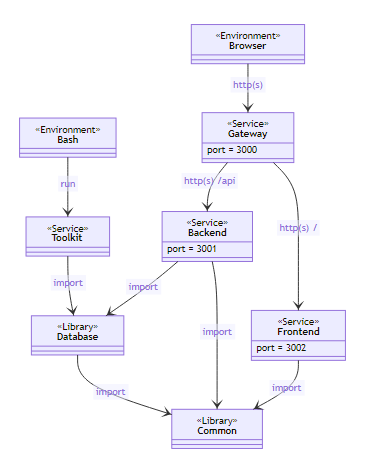
\includegraphics[width=\columnwidth]{packages-v3.png}
        \caption{Packages}
        \label{fig: packages}
    \end{figure}

    \subsubsection*{Gateway}
    The gateway runs at port 3000. It establishes a connection between the services backend, broker, worker and frontend. When the app is started the gateway serves as the entry address. It displays the frontend, which itself runs on port 3003, while the backend is running in parallel. 
  
    \subsubsection*{Frontend}
    The frontend provides an interface to make changes to the data via the offered functions of the developed API. To create the user interface React version 17 was used. It uses React states that can be altered with React hooks. The frontend communicates via HTTP requests with the backend to create, read, update and delete data with help of the API located in the backend. This communication runs with the library Axios. To display the uploaded cad models three.js was used. It offers a 3d view of the selected CAD file. The view of the model can be adjusted by zooming and rotating, as well as positioning [see Fig. \ref{fig: versionview} on page~\pageref{fig: versionview}]. The library Recharts provides a variety of different charts and graphs. Recharts is used to display a burn down chart in a specific user interface component [see Fig. \ref{fig: sprintview} on page~\pageref{fig: sprintview}].

    \subsubsection*{Backend}
    The backend of the app is built with the framework nest.js. This area of the software is the core component and provides those functions to meet the previously defined requirement specifications. Using nest.js, an API was created that interacts with the data using CRUD commands and sends it to the frontend. For that, it receives commands from the frontend and then executes the corresponding function of the API. The backend is controlled via HTTP requests. Therefore, the commands can be executed without the frontend. Good possibilities are offered by the program Postman or with Swagger. A Swagger integration was done in the backend during the development process. Swagger provides good documentation about the API and allows its functions to be executed without the frontend.

    \subsubsection*{Common}
    The package common provides the necessary interfaces for the communication of the frontend and backend. In this section the data classes like product, version, issue, etc. for the different functions are defined. 
    The rest file contains the interfaces for the HTTP requests. They define exactly which data may be sent from the frontend and which may be received again. For this purpose, the CRUD methods with transfer parameter and return value are defined in each interface of a data class.
    
    \subsubsection*{Database}
    To store the data permanently a PostgreSQL database is used. It runs in a Docker container on port 5432. The database uses the data classes defined in the interface as entities. For the object relational mapping TypeORM is used. 
    
    \subsubsection*{Toolkit}
    The toolkit package provides functionality to fill the database with test data. Based on the classes defined in the interface, the respective objects are instantiated here. These objects are filled with fictitious data to test the functionality of the app. After the objects are instantiated, they are loaded into the database. For this purpose asynchronous function calls are executed.

    \subsection*{Data model}
    The core of the software is in the backend. Via the API, the data can be manipulated using CRUD methods. This section describes the data model of the app. The necessary classes and entities are based on the interfaces in the common package. The difference between the data in the backend and in the database is that each entity class in the backend is divided into update, add and the base class. In the database, the classes are not divided. For example, the class product is mapped to a table in the database.
    
    \subsubsection*{Entities} % hier noch von den diagramm texten was raus nehmen
    The data model contains following entities [see Fig. \ref{fig: datamodel} on page~\pageref{fig: datamodel}]: User, Product, Version, Issue, Comment, Milestone, Member. At the top level of the data model is the user, who can create multiple products if he has the permission to do so. For each product versions, issues, comments, milestones and members can be created. The entity User has personal attributes like the profile picture name, email, password and the two permissions to create and change users or to create products. Finally, like any other entity, the user has a deleted flag. If a delete method is executed, this is set to true. The find and get methods of the API are implemented to search only for objects that are not deleted. When deleting, care must be taken which dependencies must also be set to deleted. If a user is deleted, no further data is removed from him. The user is only marked as deleted on the user interface. All data generated by the user will remain. All other entities are linked to the product entity. The product itself does not provide much information, because it will be filled with information later by other references. If a product is deleted, all versions, issues, comments, milestones, and members must also be set to deleted. The versions contain important information and the 3D CAD model. To create a versioning, the attributes major, minor and patch are specified for a version. The baseVersionIds are used to identify the previous version. By knowing the current version and previous version, a graphical overview can be built on the UI. Multiple issues can be added for each project. Label and text contain information about the issue. The state distinguishes between open and closed issues. So it is possible to filter for completed and not completed issues. The attribute assigneeId is a string array. Here the userIds of the users are specified who have the task to solve the issue. The milestoneId can be used to add the issue to a milestone. For each issue one or more comments can be created. These comments have a text, an author and a corresponding issue as well as the time of the post. With the attribute action an issue can be closed or reopened by the comment. For each product one or more milestones can be defined. These have a label and clear start and end dates. UserId and productId serve as foreign keys. Later it can be counted how many issues per milestone are still open or already closed. This can be used to display a graphical representation of the project progress in the frontend. For each product one or more members can be added. These members have the foreign keys productId and userId. The attribute role can have three states: manager, engineer, customer. Depending on the role, the corresponding product member has different permissions to interact with the respective product.

    \begin{figure*}[t]
        \centering
        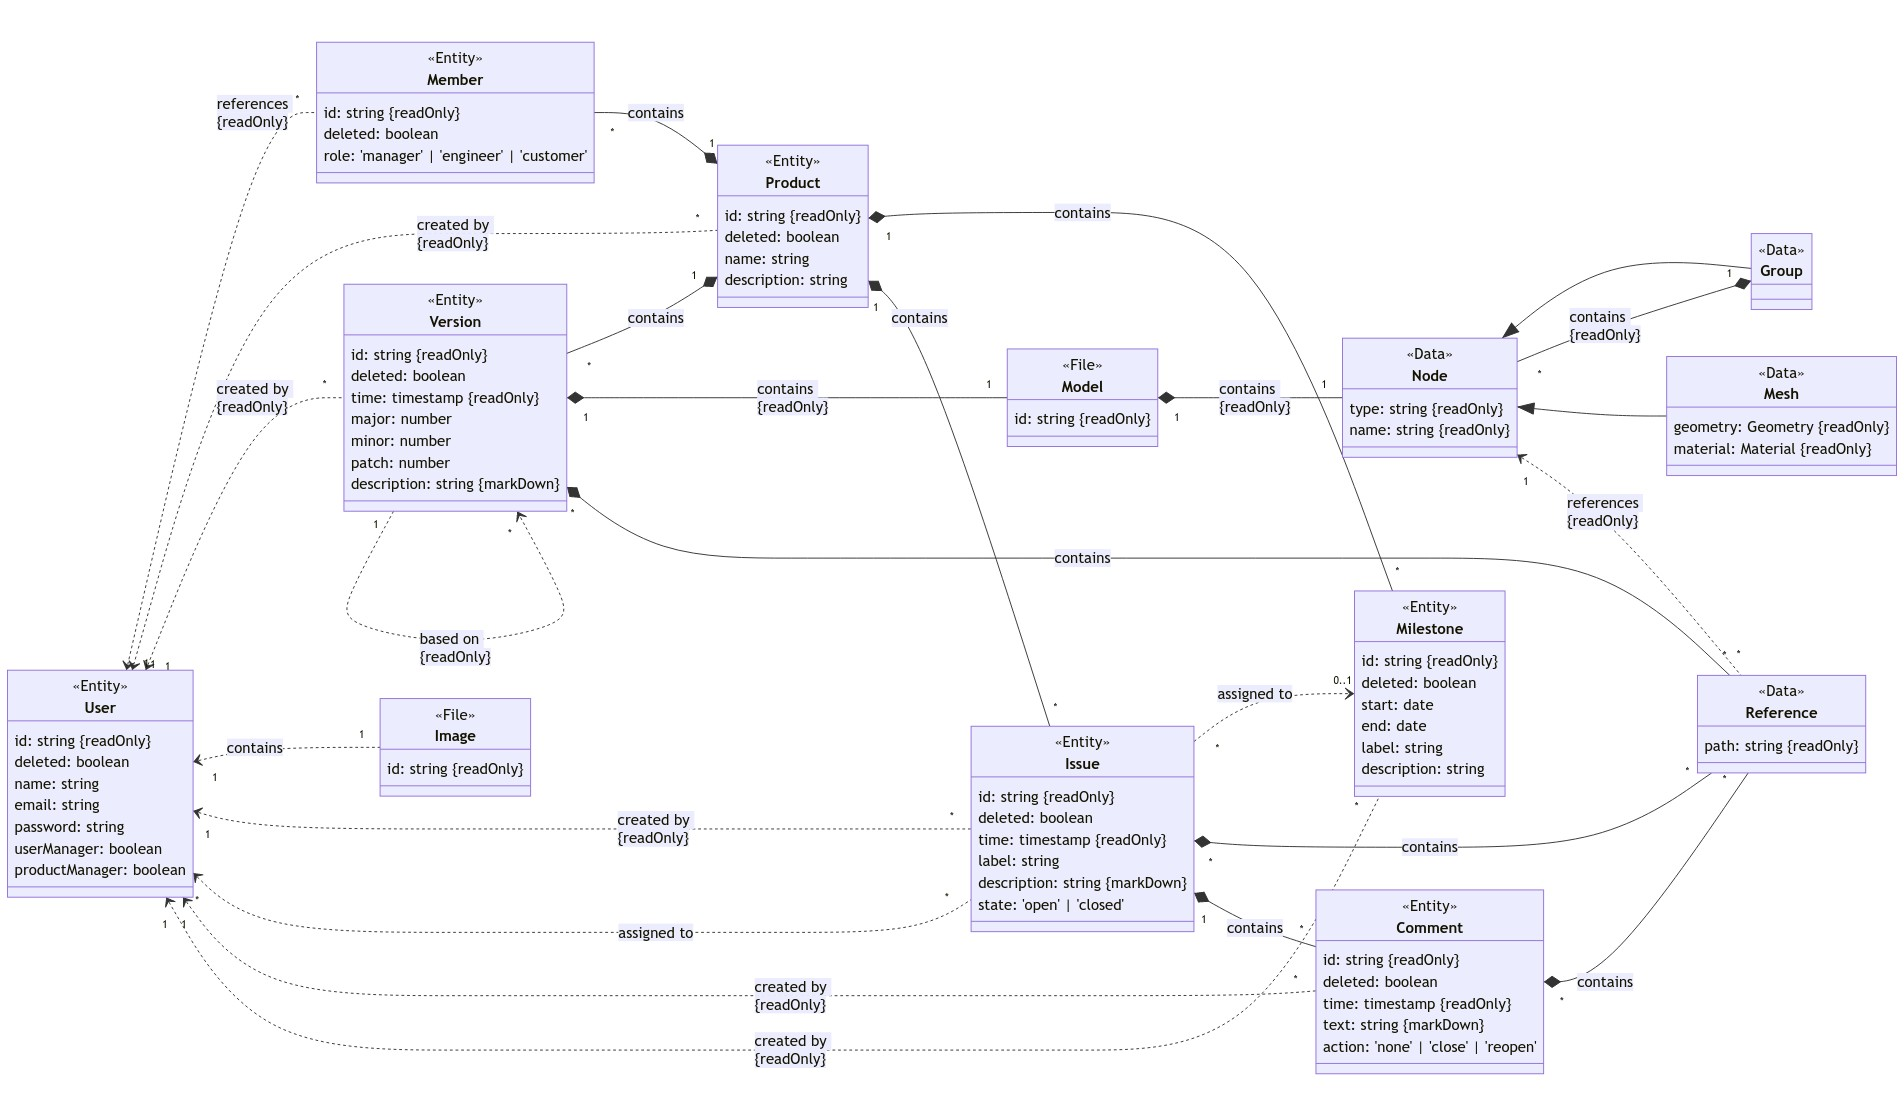
\includegraphics[width=\textwidth]{entities-v5.png}
        \caption{Data model}
        \label{fig: datamodel}
    \end{figure*}

    \subsection*{Function model} 
    The functions implemented in the API allows to create, read, update and delete data. This would not even require a graphical user interface. All functions offered by the API are called via HTTP requests. These requests can also be made via the console or other software such as Postman or Swagger. Thus, the functional model in combination with the data model is the foundation of this application. The API is built with nest.js. One rest entity contains of controller, service and module. In operation, an HTTP request is performed in the frontend. The data flows from the respective view via a request manager to a rest method, where the respective Axios request is triggered. In the backend, the nest controller receives the request and sends it on to the nest service. The nest service implements the necessary API methods to make changes to the data. These functions are all asynchronous and have a Promise as return value. After processing, the result is returned. This tunnel is provided with various permission checks to verify that the user or product member has the permission to perform this action. The interface in the common package controls the communication between frontend and backend. In the nest service the methods find, add, get, update, delete and convert are available. The convert method parses the received database object back into an object that can be further processed by the software.

    \subsubsection*{User management}
    Users can be created, modified and deleted here. The condition for this is that the respective user has the User Manager Permission. When a user is created, the associated data object is filled with the respective attributes. Permissions can be assigned to allow the new user to create and edit other users and to create products. For this the two attributes user management permission and product management permission have been added. The API offers the following methods for interaction with user objects:
    
    \begin{itemize}
        \item findUsers(query?: string, productId?: string) 
        \item addUser(data: UserAddData, file?: File)
        \item getUser(id: string)
        \item updateUser(id: string, data: UserUpdateData, file?: File)
        \item deleteUser(id: string)
    \end{itemize}

    The \texttt{findUsers} method searches for all users of the system from the database. It can be searched either via a query by user name or via the product id. The parameters query and productId are optional. Depending on which parameter is specified, the search process runs differently. The users found in the database are converted into user objects with the convert method, pushed into an array and returned. For the addUser method the transfer parameter is needed, which contains the information about the new user. The second parameter holds the profile picture and is optional. The UserAddData object is generated in normal operation via the User settings view and sent to the backend. GetUser searches for a specific user based on the userId and returns the object after conversion. UpdateUser needs the userId, the UserUpdateData object and optionally a file containing a profile picture. DeleteUser sets the deleted flag of the particular user to true. The get and find methods are implemented that way, to search for objects that are not deleted. The convert method is in each class and parses the database entities back into objects for further processing.

    \subsubsection*{Product management}
    This part of the API provides methods to make modifications to product objects. Here products can be created, modified and deleted. The following bullet points show the methods that are available for interacting with products:

    \begin{itemize}
        \item findProducts()
        \item addProduct(data: ProductAddData)
        \item getProduct(id: string)
        \item updateProduct(id: string, data: ProductUpdateData)
        \item deleteProduct(id: string)
    \end{itemize}

    The findProducts method searches in the database for all products that are not deleted. For this no passing parameter is necessary. The other methods work according to the same principle as in user management. It is searched with the corresponding productId for the object and displayed or its properties get changed. When deleting a product, it must be ensured that all objects that are attached to a product are also deleted. So if a product is deleted, all versions, issues, milestones and members must also be set to deleted.

    \subsubsection*{Version management}
    Only by referencing a version to a product it gets further descriptive properties and the 3D CAD model. Again, the API provides CRUD methods to interact with versions:

    \begin{itemize}
        \item findVersions(productId: string)
        \item addVersion(data: VersionAddData, file: File)
        \item getVersion(id: string)
        \item updateVersion(id: string, data: VersionUpdateData, file?: File)
        \item deleteVersion(id: string)
    \end{itemize}

    Unlike user management, a file must be specified when a version is created. This is an STL file, which is then stored locally. This CAD model can be exchanged when updating the version.

    \subsubsection*{Issue management} 
    These methods are available to create, read, update and delete issues:
    \begin{itemize}
        \item findIssues(productId: string, milestoneId?: string, state?: 'open' or 'closed')
        \item addIssue(data: IssueAddData)
        \item getIssue(id: string)
        \item updateIssue(id: string, data: IssueUpdateData)
        \item deleteIssue(id: string)
    \end{itemize}

    The findIssues method can search for issues in the database in several ways. An issue is always connected to a product. Thus, the productId must always be passed. Aditionally, the milestoneId parameters can be given to the method to search for issues that belongs to a specific milestone. The state parameter allows to filter the issues by closed and open. This is especially useful to be able to filter for completed or uncompleted tasks for  the purpose of product management. When deleting issues, all comments belonging to the respective issue must also be deleted.

    \subsubsection*{Comment management}
    The following list shows the methods that can be performed to interact with the comment objects:
    \begin{itemize}
        \item findComments(issueId: string)
        \item addComment(data: CommentAddData)
        \item getComment(id: string)
        \item updateComment(id: string, data: CommentUpdateData)
        \item deleteComment(id: string)
    \end{itemize}

    An issue can have one or more comments. These comments are bound to an issue and the issue is bound to a product. The findComments method stores all comments for a given issueId in an array and returns it. 

    \subsubsection*{Milestone management}
    Milestones are a container that can be filled with issues by reference. The CRUD methods are listed below:
    \begin{itemize}
        \item findMilestones(productId: string)
        \item addMilestone(data: MilestoneAddData)
        \item getMilestone(id: string)
        \item updateMilestone(id: string, data: MilestoneUpdateData)
        \item deleteMilestone(id: string)
    \end{itemize}

    The methods have analogous purposes as already with the other data objects. When deleting a milestone, it must be ensured that the references to the linked issues are removed. For this purpose, the milestoneId attribute of each associated issue is set to null again.

    \subsubsection*{Member management}
    The API provides the following methods for member management:

    \begin{itemize}
        \item findMembers(productId: string, userId?: string)
        \item addMember(data: MemberAddData)
        \item getMember(id: string)
        \item updateMember(id: string, data: MemberUpdateData)
        \item deleteMember(id: string)
    \end{itemize}

    Members are always linked to the respective product. Additionally, the userId can be used to search for one specific member. The findMembers method returns an array of members that can then be displayed on the user interface.
    The other methods are similar to those of the other entities

    \subsection*{Permission model}
    The permission model offers a number of possible restrictions on the platform so that not every user has all freedoms. This is especially important when cooperating with customers. The customer should only have the possibility to evaluate existing products. For this he can see the products he is registered for and use the given product management functions. Creating new users and products should only be possible by the developers of the respective product. They also organize the rights of each user. The permission model is divided into two levels. The first level is the user level and the second level is created by the product members. This system is deeply integrated in the backend. Each method of the API checks with each call whether the respective user or the member role has the necessary permissions for the execution. All permission of the respective user and member roles are stored in a separate permissions.ts file. 

    \subsubsection*{User level}
    The User entity has the two attributes user management permission and product management permission. Only a user who has the user management permission can see the Users button in the upper right corner of the frontend and create or edit users there. With the product management permission it is possible to create new products. If a new product is created, the respective user is automatically also a product member and receives the member role manager. The permissions of each user can be adjusted afterwards in the user settings [see Fig. \ref{fig: usersettingsview} on page~\pageref{fig: usersettingsview}]. So it is possible to give multiple users the permissions for user administration and product administration. For example, a user and product manager can exist for each department The following table [see Fig. \ref{tab: userlevelpermissions} on page~\pageref{tab: userlevelpermissions}] shows the division of permissions into user management and product management on user level.

    \begin{figure}[h]
        \centering
        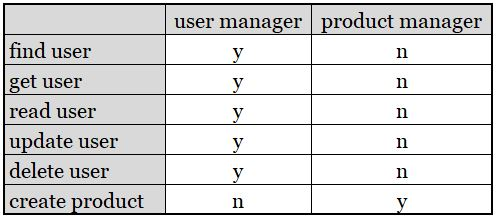
\includegraphics[width=\columnwidth]{userlevelpermissions.JPG}
        \caption{Permissions on user level}
        \label{tab: userlevelpermissions}
    \end{figure}

    \subsubsection*{Member level}
    For permission management at member level, three roles are provided. These roles are: manager, engineer and customer. The manager is the one who created the product and has the permission to add more members. So he can add more managers, who in turn have all the rights over the management of the product. This is useful when the product development covers several departments. The second role is the engineer. He is involved in the product development process. He has no rights to change the product or its members. However, he can freely create and edit versions, issues, comments and milestones. The last role is the customer who has the possibility to observe the product development process. He can follow the progress of the project, but has no permission to change anything on the platform. In the current version of the software the rights of the customer are still very strict. The permission system is implemented in such a way that it can be changed with few adjustments. If the customer needs writing permissions, this can be easily changed in the code. For this purpose, there is a separate file in the backend, which implements exactly these two tables for the permission management. The corresponding table [see Fig. \ref{tab: memberlevelpermissions} on page~\pageref{tab: memberlevelpermissions}]  shows an overview of the respective permissions on member level.

    \begin{figure}[h]
        \centering
        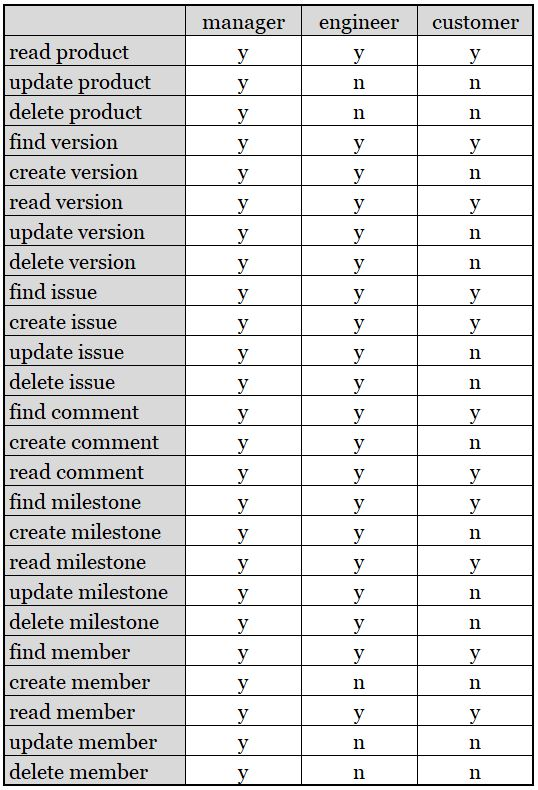
\includegraphics[width=\columnwidth]{memberlevelpermissions.JPG}
        \caption{Permissions on member level}
        \label{tab: memberlevelpermissions}
    \end{figure}
    
    \subsection*{Interface model} 
    The user interface provides a convenient way to interact with the functional model to modify and display data. For the frontend the library React.js version 17 was used. The data is managed in react states and manipulated with react hooks. Typescript was used for programming. The pages were designed with simple CSS without additional tools. The user interface offers a consistent design, which runs through the entire system. The header of the user interface offers three buttons. A click on ProductBoard leads back to the start page. On the right side there is the user administration and the currently logged-in user. The button to view the users is only visible if the current user has the user management permission. The rest of the page below the header adapts to the corresponding content.

    \subsubsection*{Start page}
    After a successful login with username and password you will see the start page. This page lists all available products in a table [see Fig. \ref{fig: startpage} on page~\pageref{fig: startpage}]. For each product in the table a preview is shown. The other columns show the attributes Owner, Name, Description, Versions, Issues and Members. The X on the right provides the possibility to delete the corresponding product. The owner is the person who created the product. Name and Description are defined when the product is created and can be changed later in the Product Settings [see Fig. \ref{fig: productsettingsview} on page~\pageref{fig: productsettingsview}]. The columns on the right show how many versions exist for this product, how many issues have been created and how many members have access to the product. By clicking on New product you get to a separate page where you can add a new product [see Fig. \ref{fig: newproductview} on page~\pageref{fig: newproductview}]. This button is only visible when the corresponding user has product management permission. After entering name and description the new product appears in the product list on the start page. Only by creating a new version for a product a CAD model with further information is added.

    \begin{figure}[h]
        \centering
        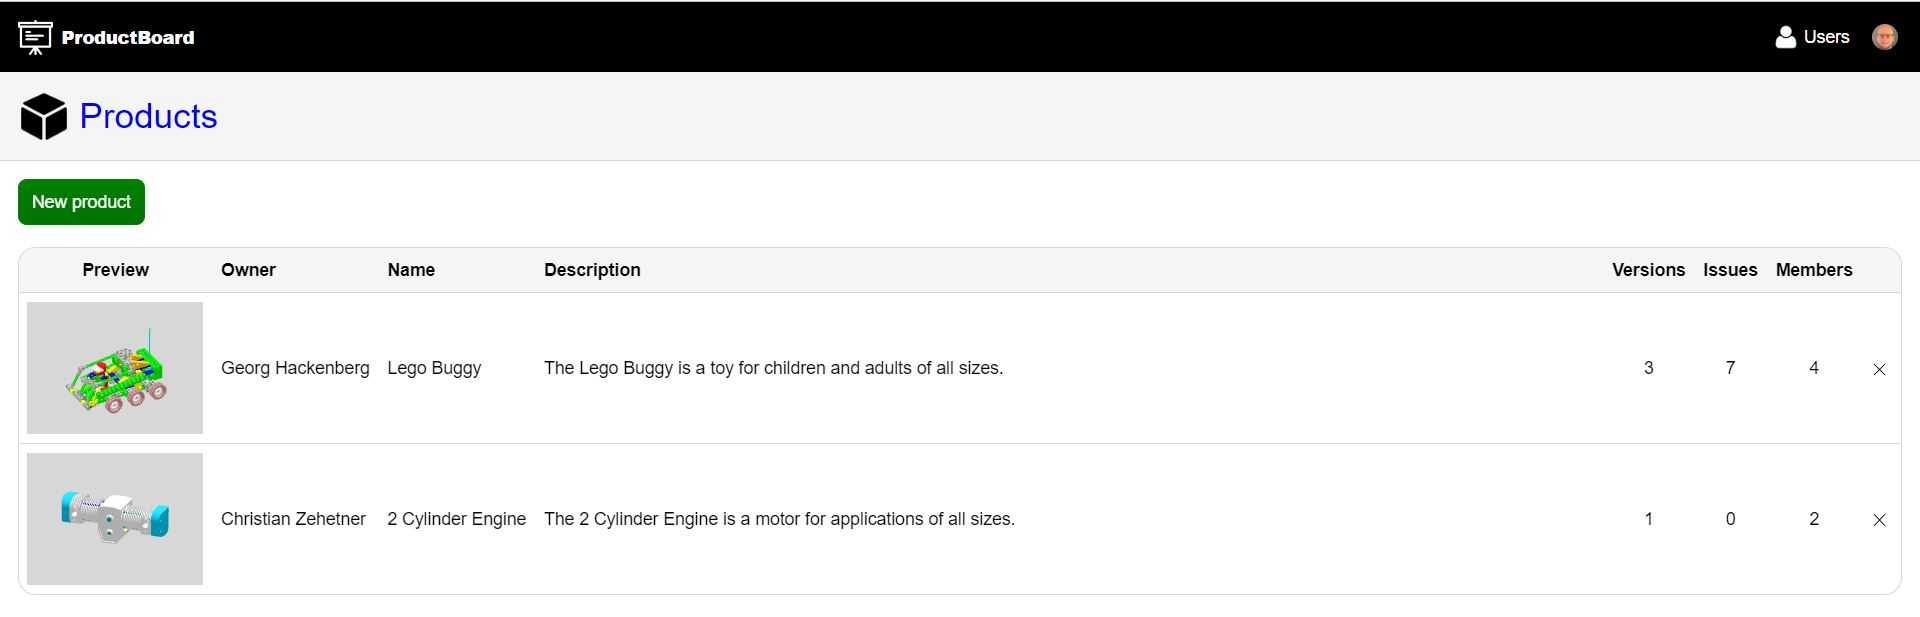
\includegraphics[width=\columnwidth]{startpage.JPG}
        \caption{Startpage}
        \label{fig: startpage}
    \end{figure}

    \begin{figure}[h]
        \centering
        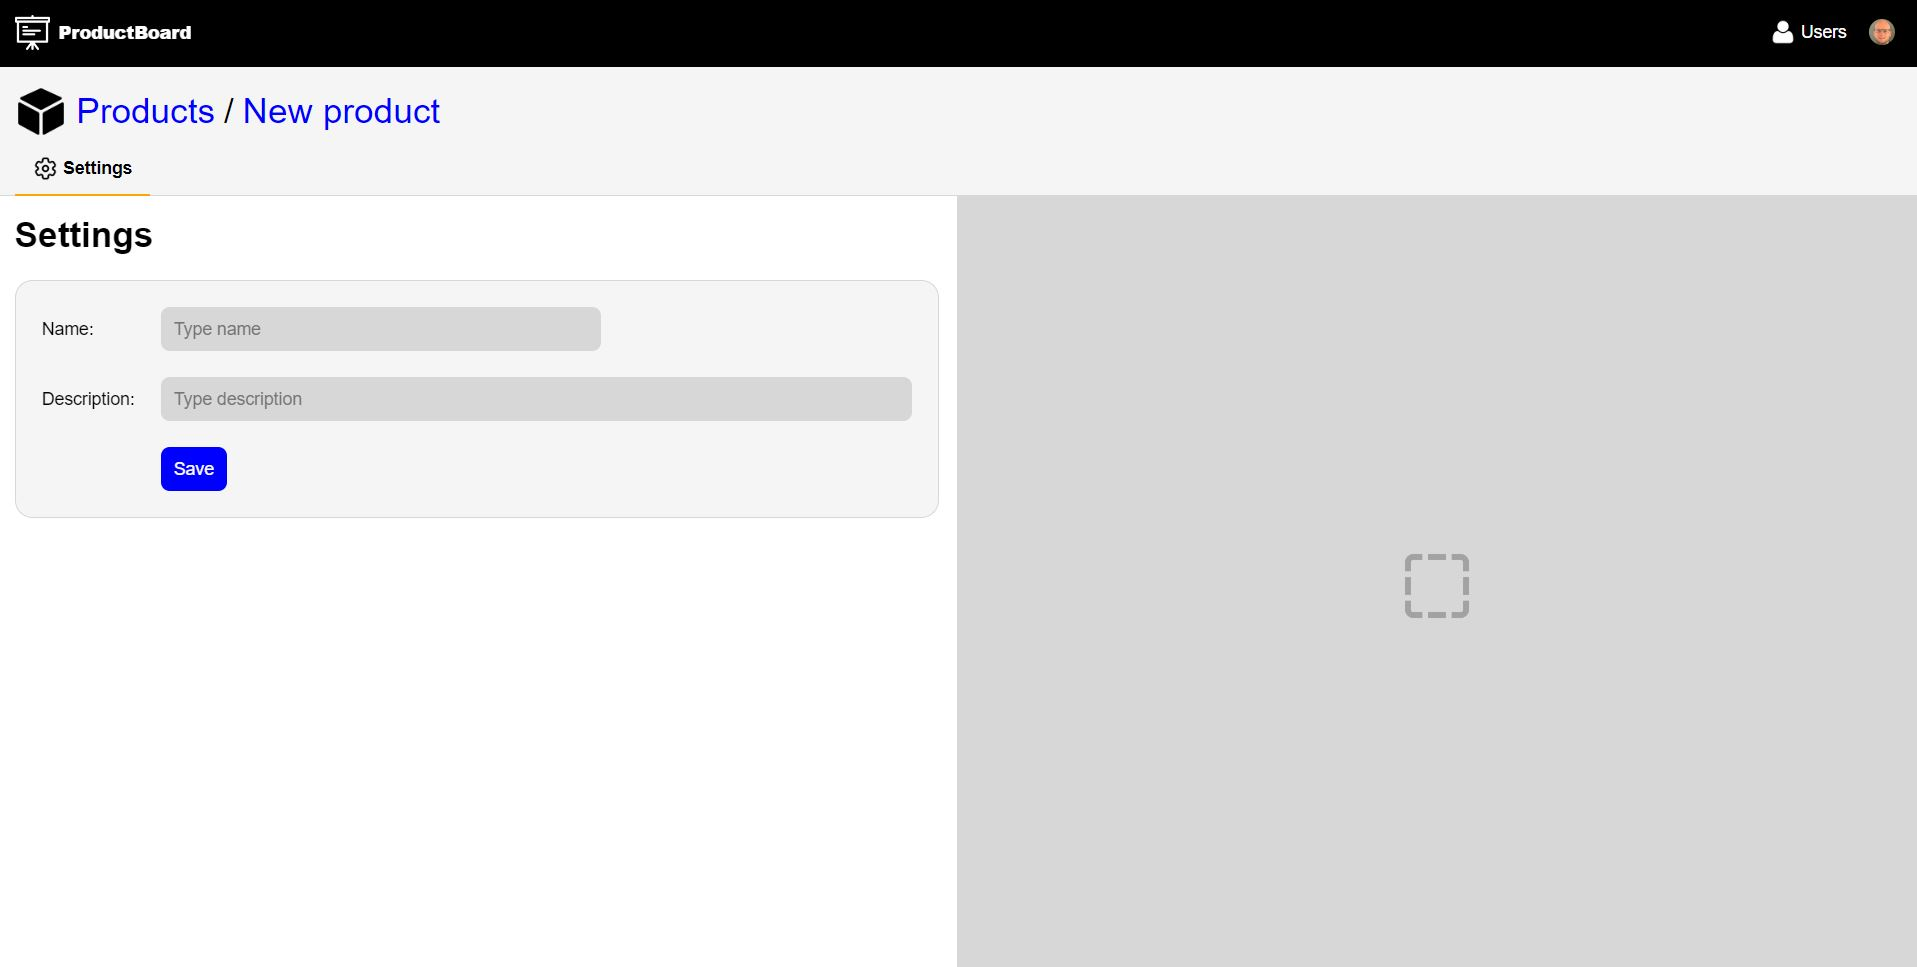
\includegraphics[width=\columnwidth]{newproductview.JPG}
        \caption{Add new product}
        \label{fig: newproductview}
    \end{figure}

    \subsubsection*{User management}
    This view is only accessible if the active user also has the authorization. By clicking on Users this page is called. If the user does not have user management permission, the button is not visible. On this page all users with profile picture, name, email and permissions are displayed [see Fig. \ref{fig: usermanagement} on page~\pageref{fig: usermanagement}]. You can delete a user by clicking on the X on the right side. If a user is clicked on, he can be edited via the User settings. The button New user also leads to the user settings where you can provide information and create a new user by clicking on the save button [see Fig. \ref{fig: usersettingsview} on page~\pageref{fig: usersettingsview}]. Save leads back to the user overview and shows the new or changed user in the table.
    
    \begin{figure}[h]
        \centering
        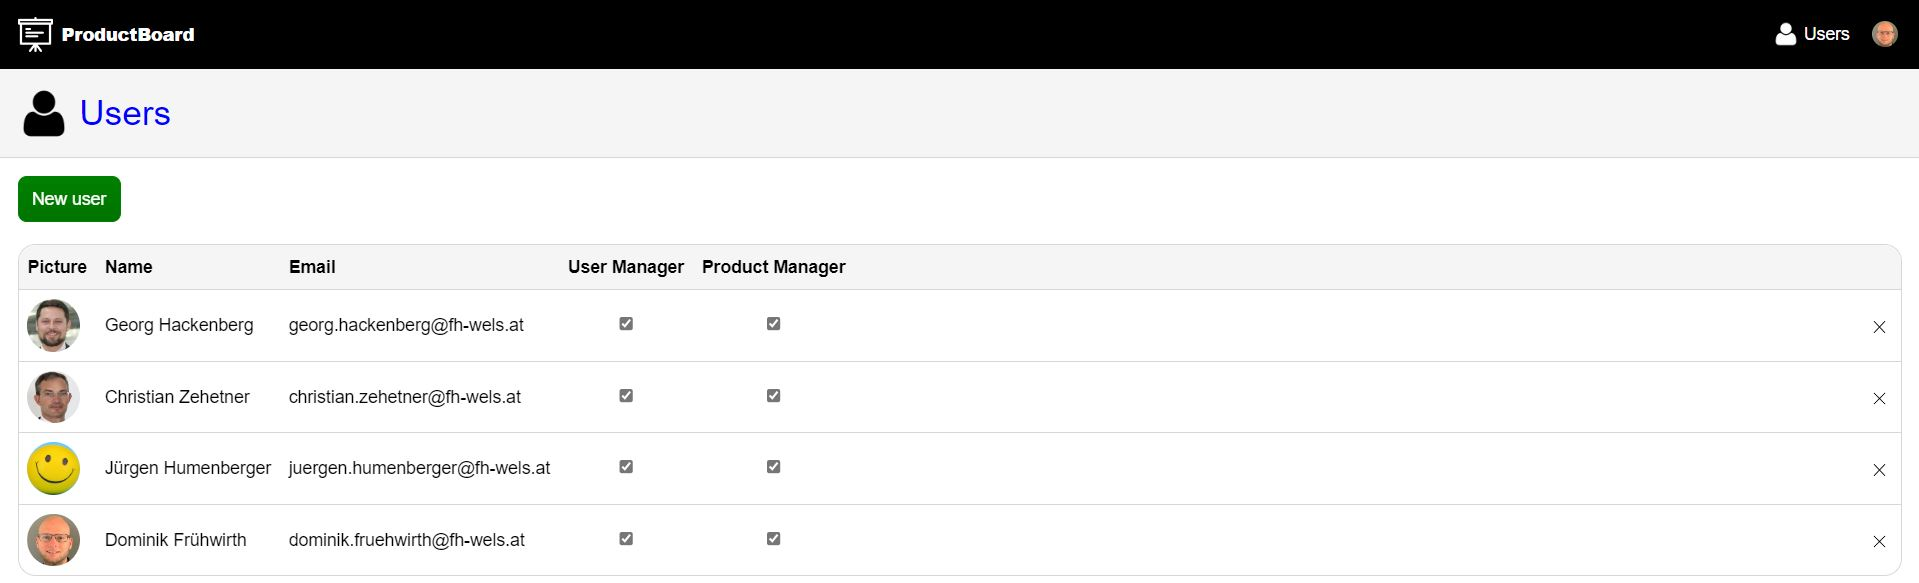
\includegraphics[width=\columnwidth]{usermanagement.JPG}
        \caption{User management}
        \label{fig: usermanagement}
    \end{figure}

    \begin{figure}[h]
        \centering
        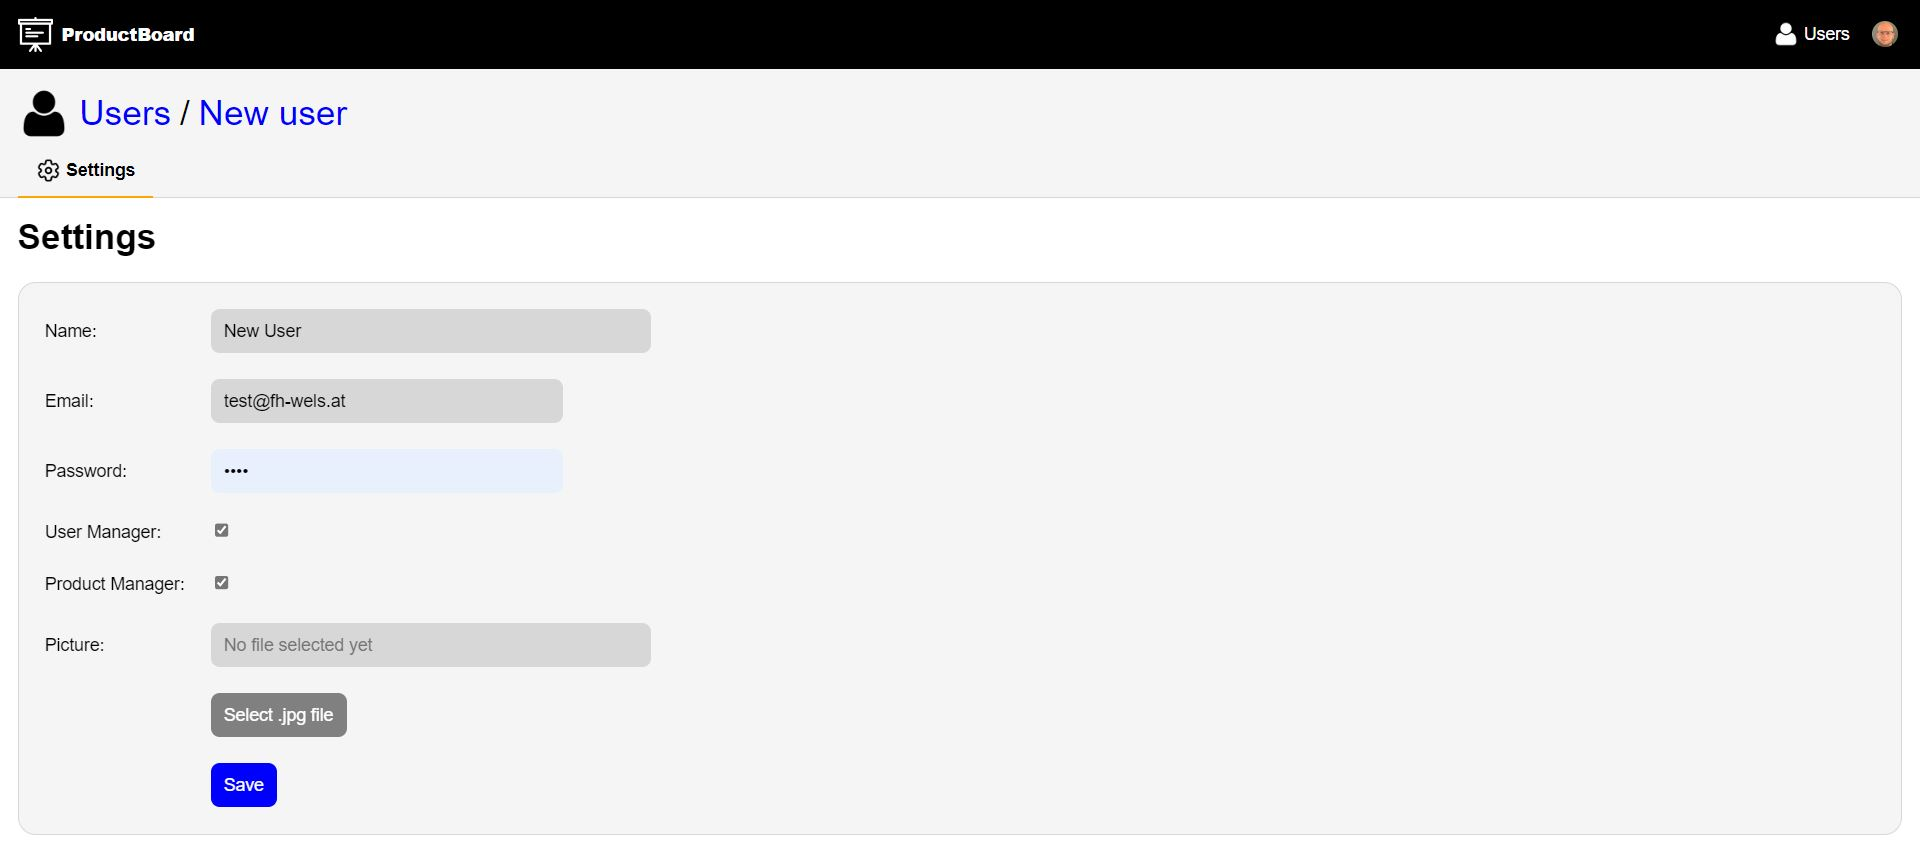
\includegraphics[width=\columnwidth]{usersettingsview.JPG}
        \caption{User settings}
        \label{fig: usersettingsview}
    \end{figure}

    \subsubsection*{Version view}
    Clicking on a product takes you to the version view [see Fig. \ref{fig: versionview} on page~\pageref{fig: versionview}]. You can also use the toolbar to jump to other pages such as Issues, Milestones Members or Settings. Next to the links a number in brackets shows how many objects per category have already been created. The left side of the Version view shows the created versions. On the left side there is a tree structure similar to Git. In the middle is the corresponding version number with the owner of the version inclusive email and a short description. Each version offers a preview. By clicking on the respective version, the 3D view on the right side also changes and shows the selected model. The 3D view was built with three.js. It allows to rotate, move and zoom the model. With a click on New version you get to the version settings [see Fig. \ref{fig: versionsettingsview} on page~\pageref{fig: versionsettingsview}]. There you can enter information for a new version and select an STL file. Depending on the selected base version, the version view shows the new version with the corresponding new tree structure after pressing the Save button.
    
    \begin{figure}[h]
        \centering
        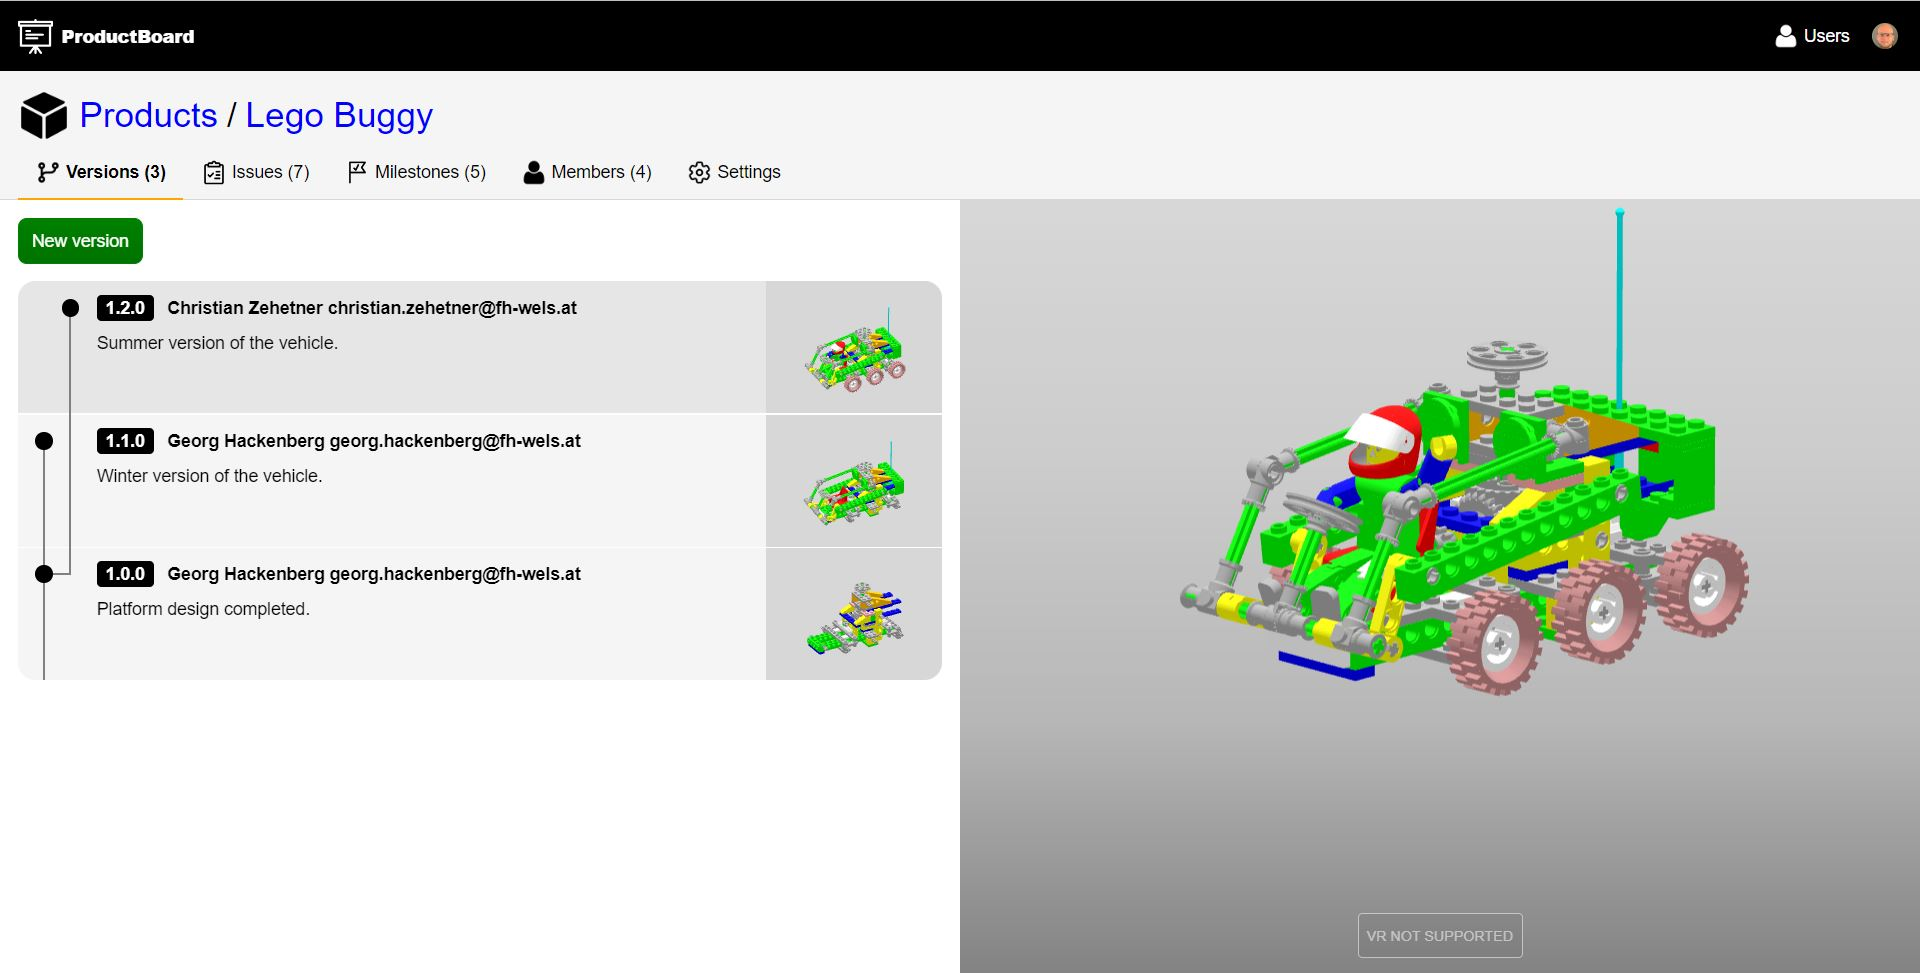
\includegraphics[width=\columnwidth]{versionview.JPG}
        \caption{Version view}
        \label{fig: versionview}
    \end{figure}

    \begin{figure}[h]
        \centering
        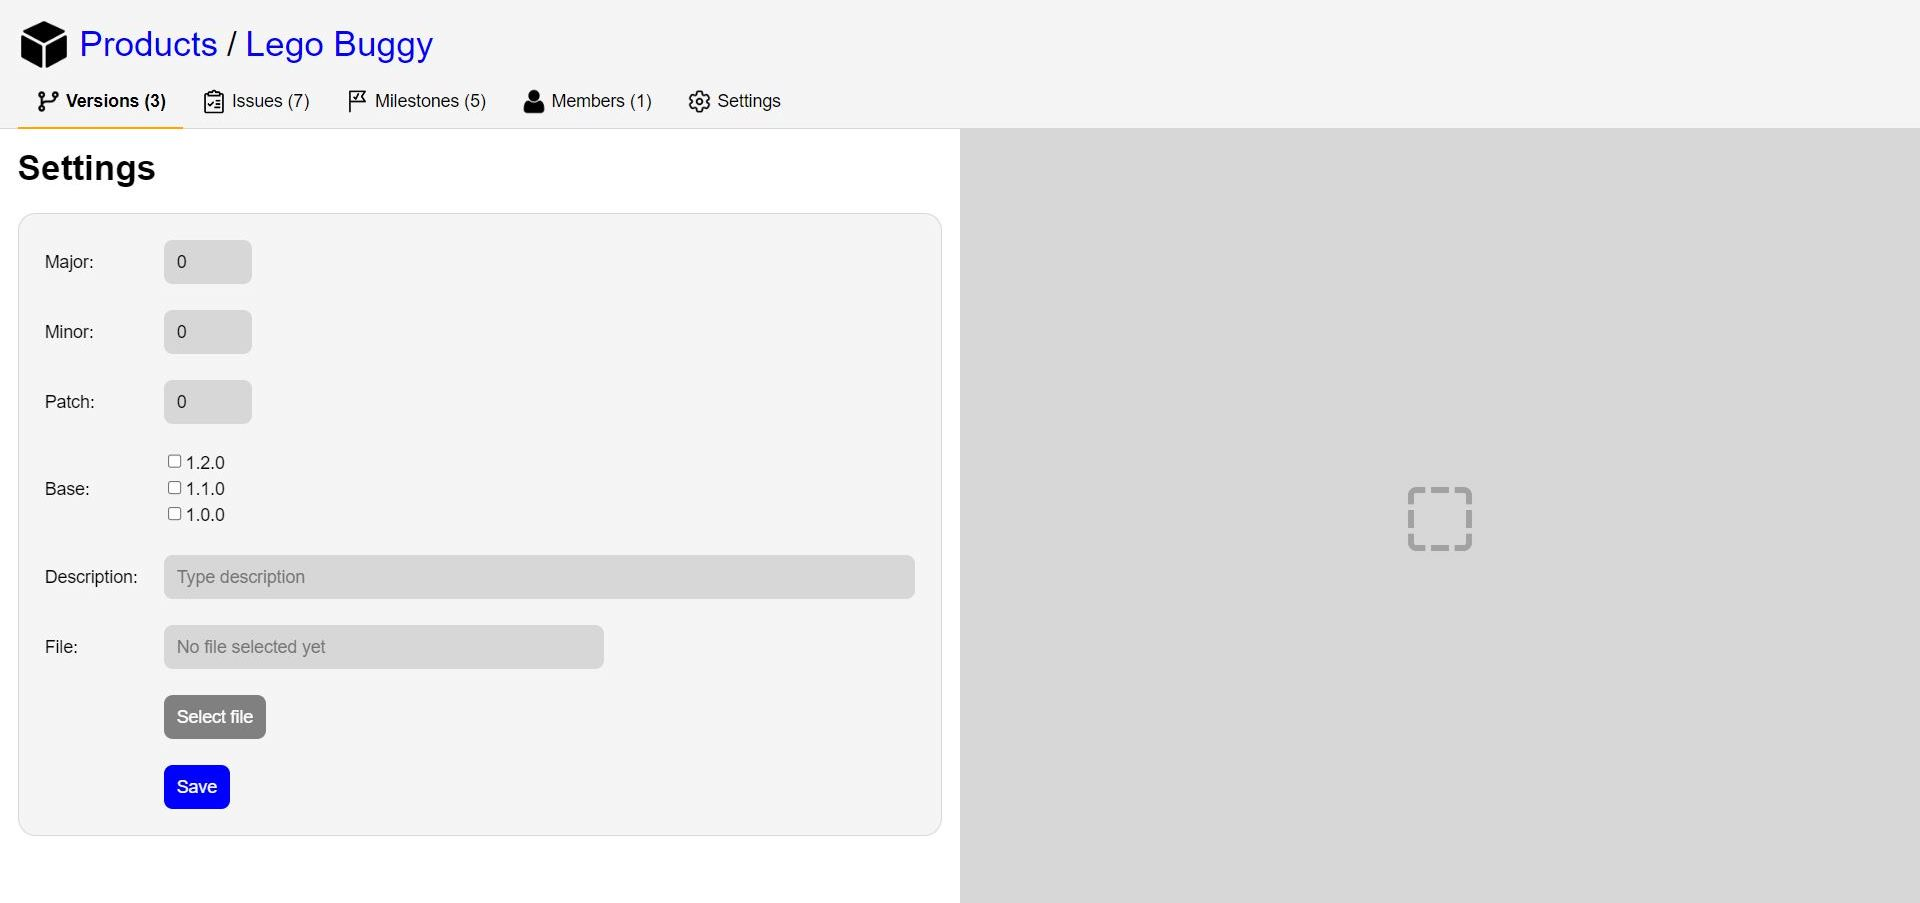
\includegraphics[width=\columnwidth]{versionsettingsview.JPG}
        \caption{Versionsettings view}
        \label{fig: versionsettingsview}
    \end{figure}

    \subsubsection*{Issue view}
    By clicking on the Issues link, you access the Issue view [see Fig. \ref{fig: issueview} on page~\pageref{fig: issueview}]. Here the created issues are displayed in a table. The two buttons Open Issues and Closed Issues can be used to filter the list accordingly. The table shows the reporter who created the issue, the associated label, the assignees and how many comments and marked parts are in the conversation channel. The Issue settings view allows to create new issues for the product [see Fig. \ref{fig: issuesettingsview} on page~\pageref{fig: issuesettingsview}]. The label, the text, the milestone and the assignees can be defined. An existing milestone can be selected with the dropdown menu. An issue must not be assigned to a milestone. This choice lies by the user. The Save button closes the settings, and you return to the Issues view where the new issue is visible. All views with 3D View offer the possibility to select a desired version for viewing. In the version view the version can be clicked directly. In the other views the version can be selected via a dropdown menu. This menu is located in the upper left corner of the 3D View.
    
    \begin{figure}[h]
        \centering
        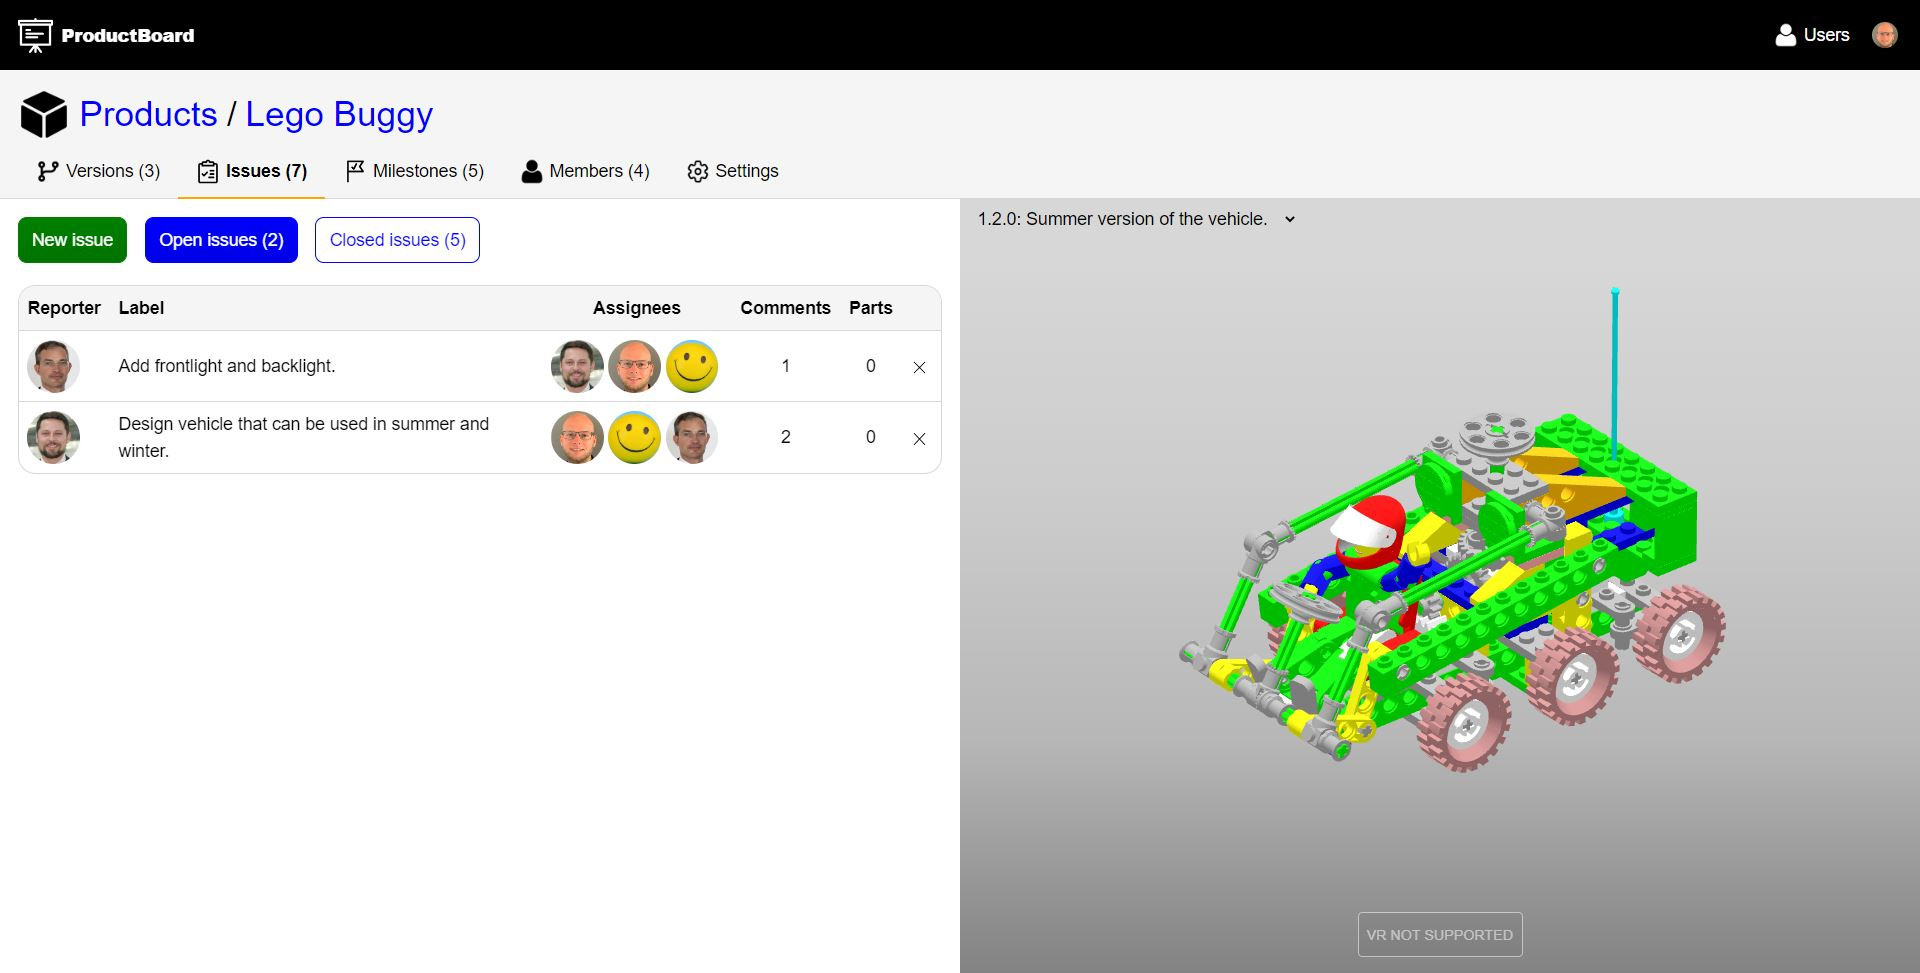
\includegraphics[width=\columnwidth]{issueview.JPG}
        \caption{Issue view}
        \label{fig: issueview}
    \end{figure}

    \begin{figure}[h]
        \centering
        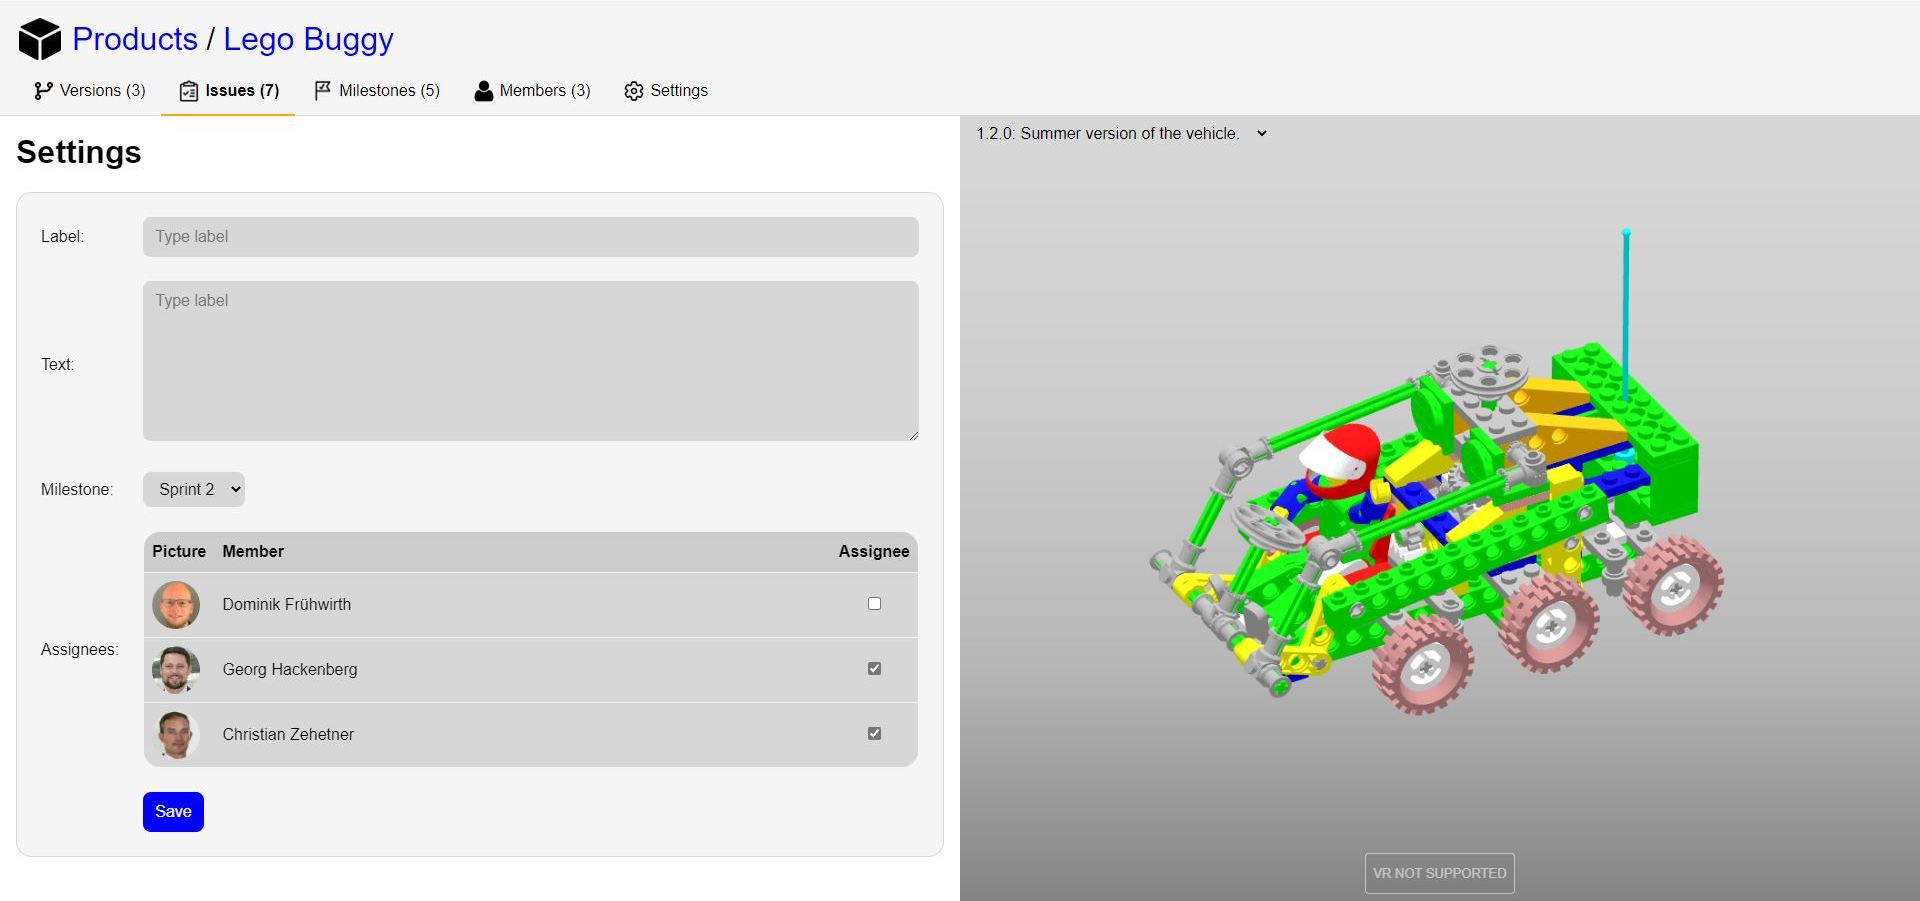
\includegraphics[width=\columnwidth]{issuesettingsview.JPG}
        \caption{Issuesettings view}
        \label{fig: issuesettingsview}
    \end{figure}

    \subsubsection*{Comment view}
    Clicking on an issue in the Issue view opens the corresponding Comment view [see Fig. \ref{fig: commentview} on page~\pageref{fig: commentview}]. Here you have the possibility to discuss the issue. You can click on a component of the 3D model in the Comment view to reference a component [see Fig. \ref{fig: commentselectedpartview} on page~\pageref{fig: commentselectedpartview}]. If a post is created or a part is selected in the comment view, the corresponding counter in the issue view table is increased. A comment can be used to close an issue by clicking Close. This issue will then be found in Closed Issues in the Issue view. With the comment function it is also possible to reopen the issue in the same way. The Close button displays the text Reopen when an issue is closed. In the upper right corner of the Comment view there is a button to edit the selected issue. For example, the issue can be assigned to another Milestone or other attributes can be changed [see Fig. \ref{fig: issuesettingsview} on page~\pageref{fig: issuesettingsview}]. A click on Save makes the changes visible in the Issue view.

    \begin{figure}[h]
        \centering
        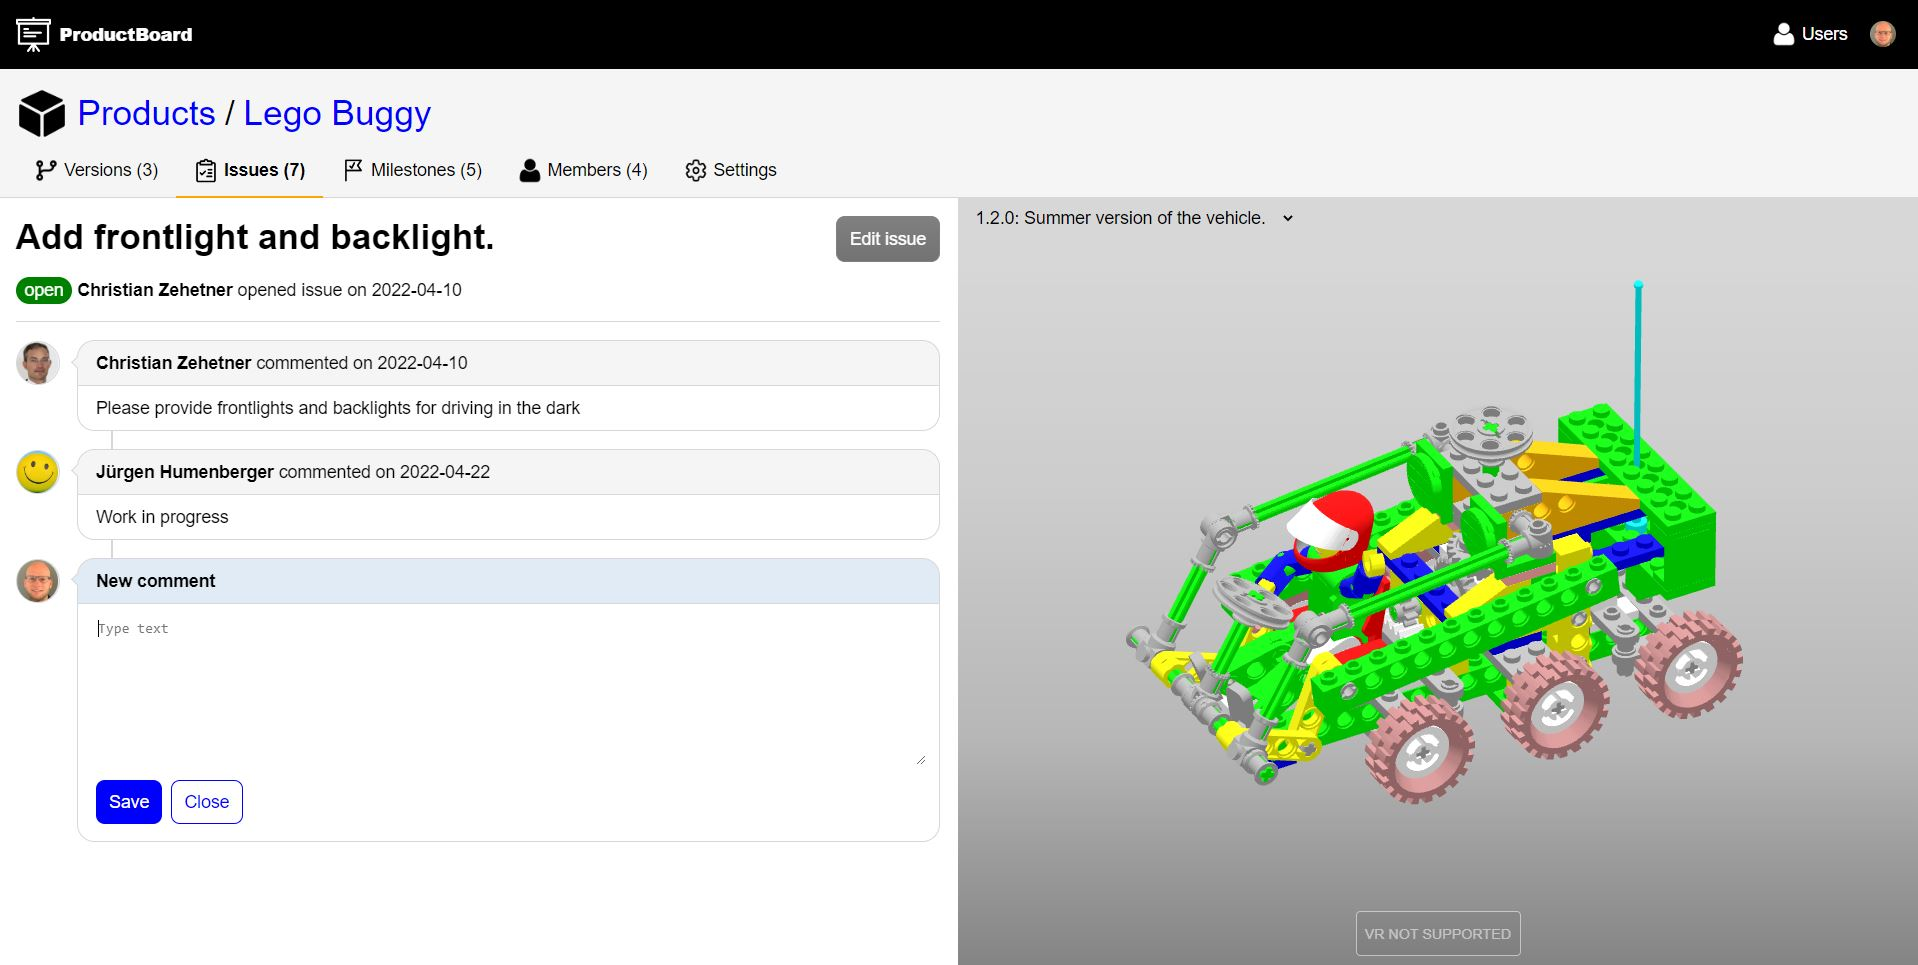
\includegraphics[width=\columnwidth]{commentview.JPG}
        \caption{Comment view}
        \label{fig: commentview}
    \end{figure}

    \begin{figure}[h]
        \centering
        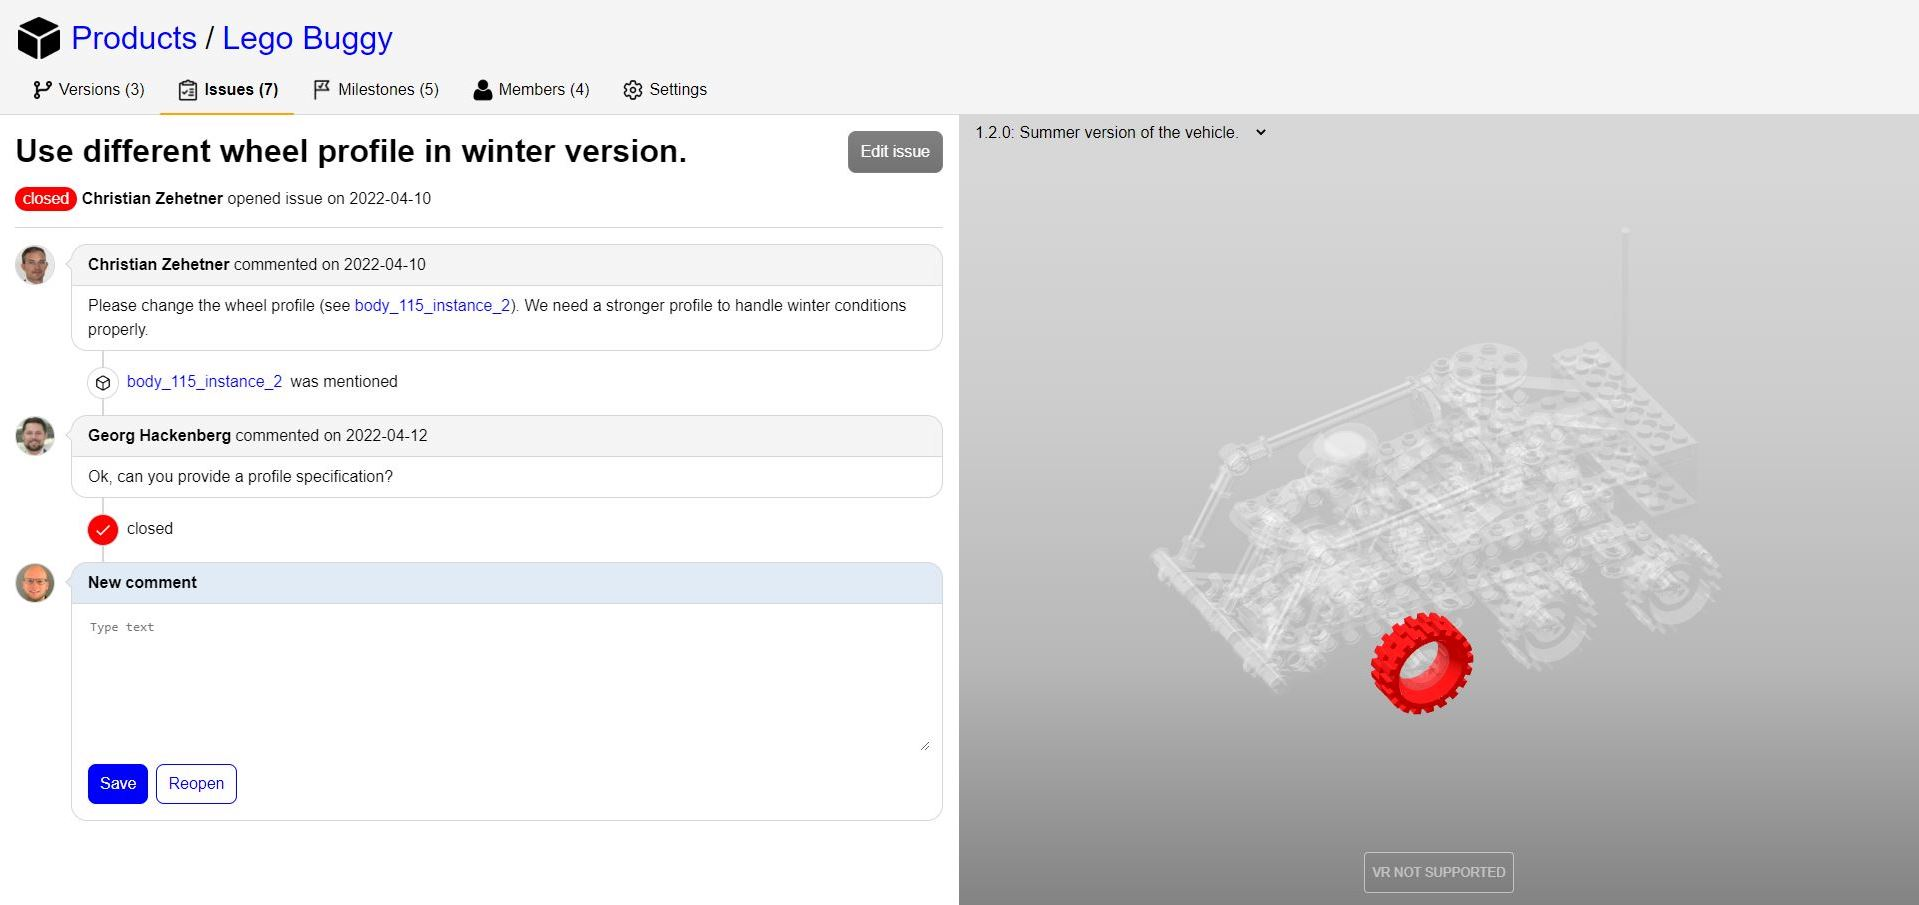
\includegraphics[width=\columnwidth]{commentselectedpartview.JPG}
        \caption{Selected part}
        \label{fig: commentselectedpartview}
    \end{figure}

    \subsubsection*{Milestone view}
    The Milestone view can be accessed via the Milestones link [see Fig. \ref{fig: milestoneview} on page~\pageref{fig: milestoneview}]. A table shows who created the milestone, its name, start date, end date and the progress like open and closed issues. For each milestone two progress bars are displayed. The first one shows the date progress and the second one the issue progress. If a milestone is selected, a table with the attached issues is displayed [see Fig. \ref{fig: sprintview} on page~\pageref{fig: sprintview}]. This table is identical to the one in the Issue view. Here you can also filter by open and closed issues. On the right side a burn down chart is displayed which shows the current progress of the milestone. The chart shows the start date, the end date, the number of issues and the progress until the current day. A click on New Milestone or Edit Milestone leads to the Milestone Settings [see Fig. \ref{fig: milestonesettingsview} on page~\pageref{fig: milestonesettingsview}]. Here the attributes of a milestone can be adjusted and saved. The new or edited Milestone than show up in the Milestone view.

    \begin{figure}[h]
        \centering
        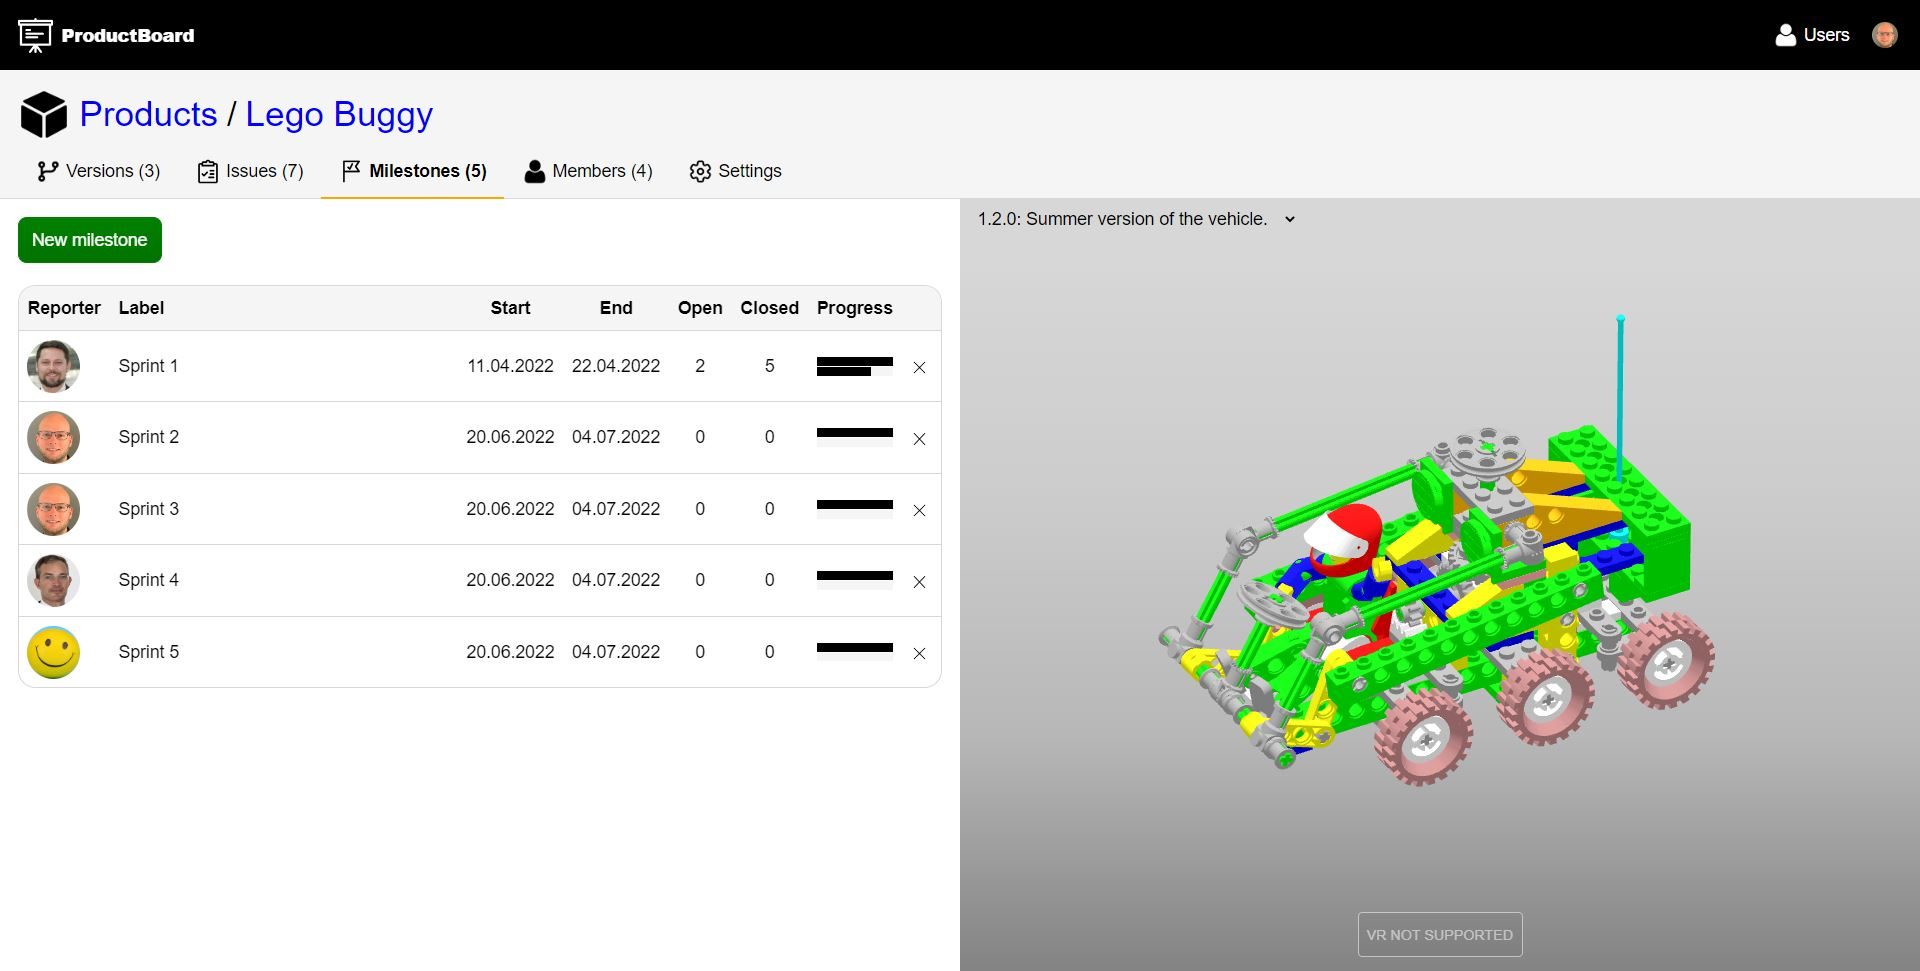
\includegraphics[width=\columnwidth]{milestoneview.JPG}
        \caption{Milestone view}
        \label{fig: milestoneview}
    \end{figure}

    \begin{figure}[h]
        \centering
        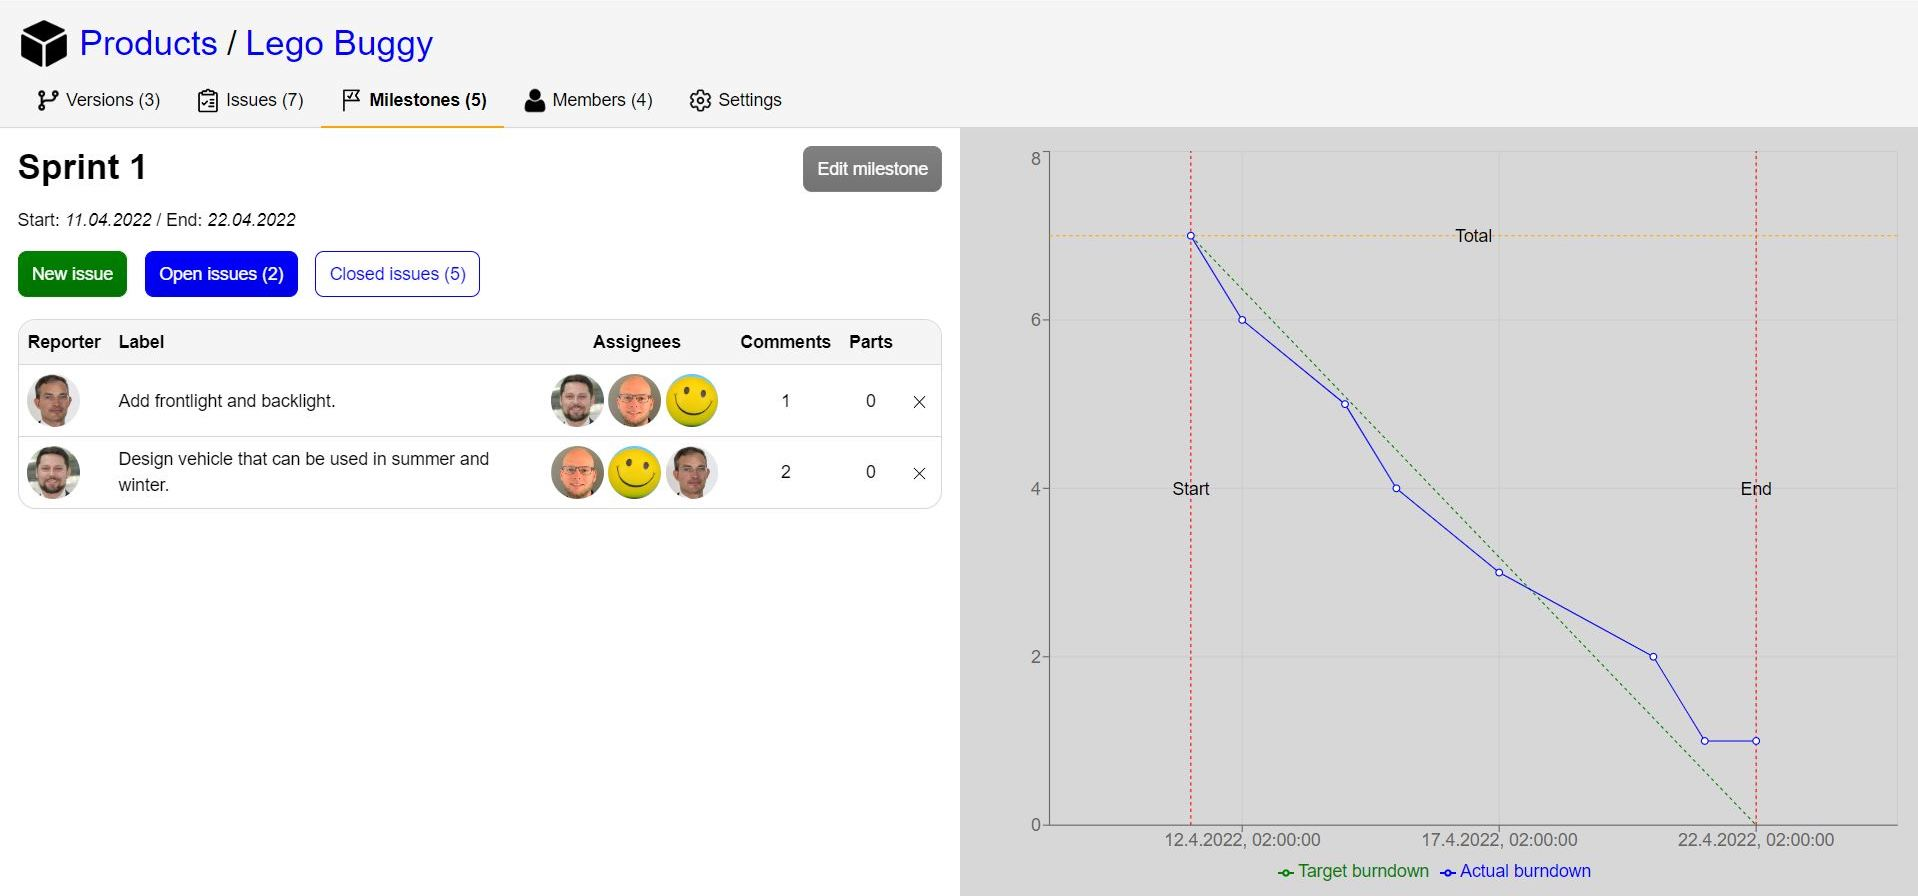
\includegraphics[width=\columnwidth]{sprintview.JPG}
        \caption{Sprint view}
        \label{fig: sprintview}
    \end{figure}

    \begin{figure}[h]
        \centering
        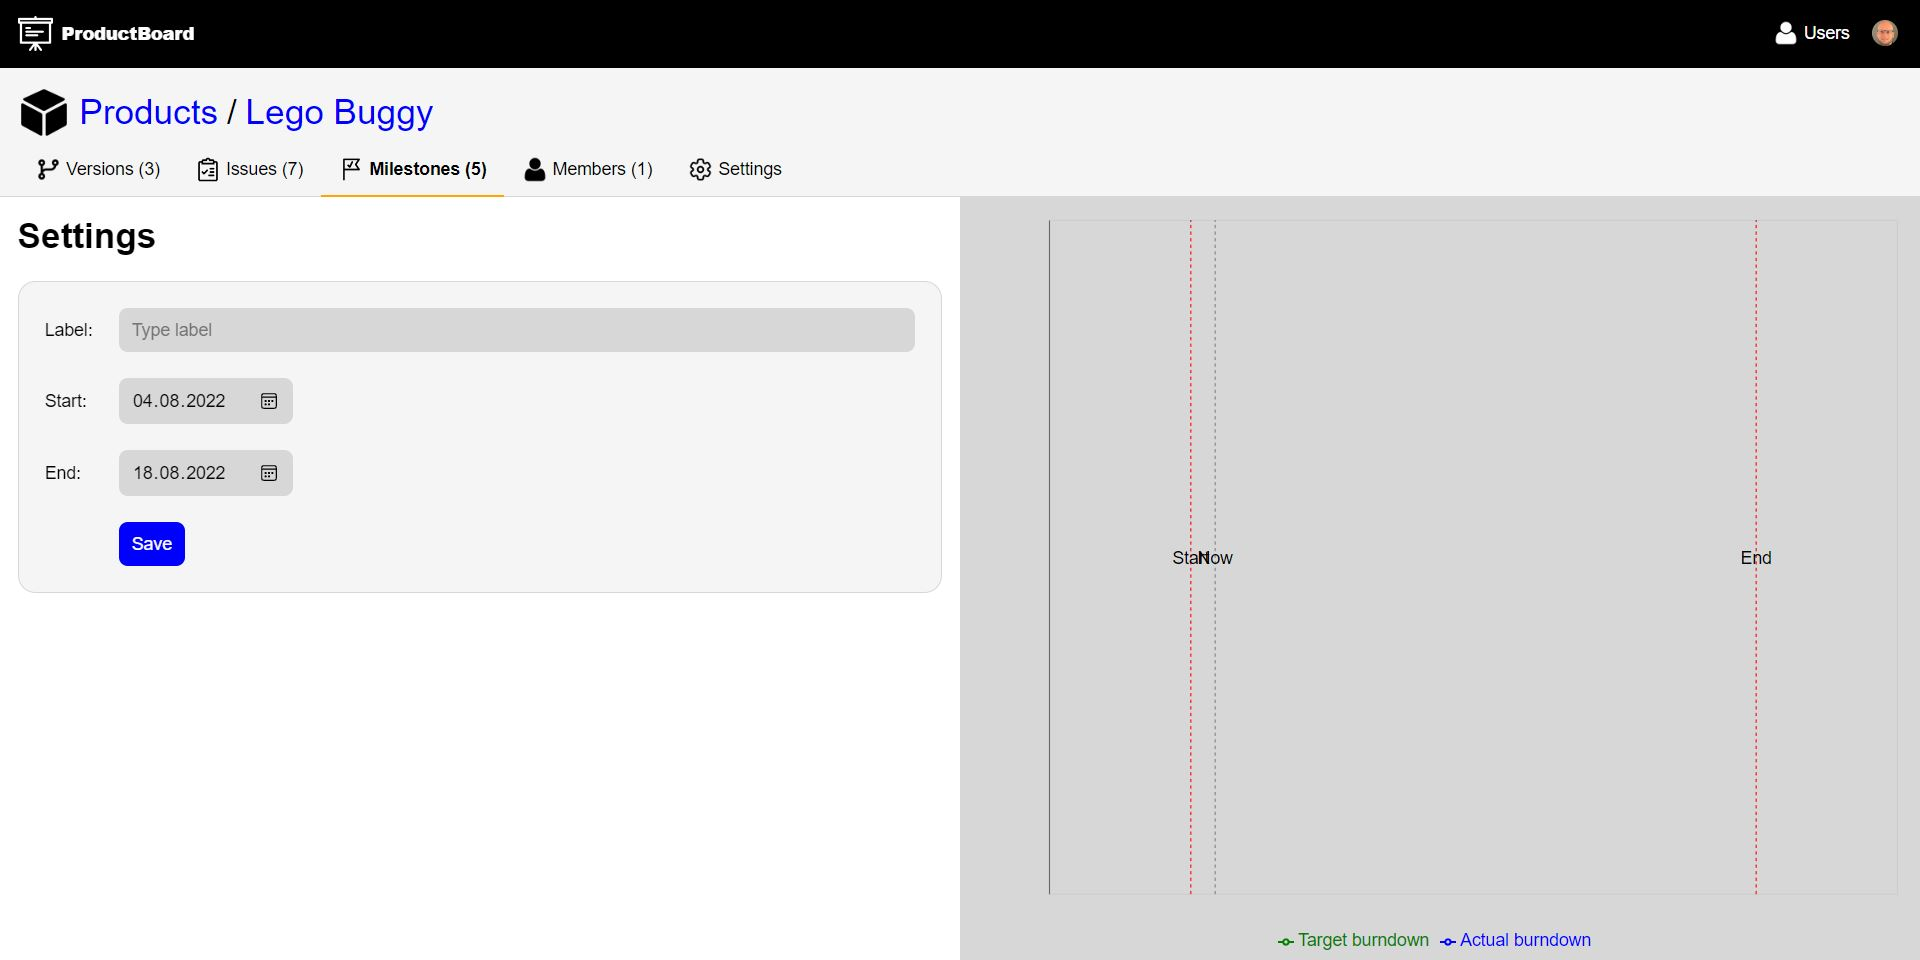
\includegraphics[width=\columnwidth]{milestonesettingsview.JPG}
        \caption{Milestone Settings view}
        \label{fig: milestonesettingsview}
    \end{figure}

    \subsubsection*{Member view}
    To distribute the rights for a product, members are added to an existing product via the user interface. In the member view, a table shows all members who have access to the selected product [see Fig. \ref{fig: memberview} on page~\pageref{fig: memberview}]. The table shows the user picture and the name of the user. The column Role defines which rights the respective member has. At the moment there are three roles: manager, engineer, customer. As with every overview table, objects can be deleted from the list by clicking on the X button. The button New Member leads to the Member settings. Here you can enter the name of a potential member into a text field. When typing, a list appears in the lower area that filters for each new letter. If you click on a user from the list, this user is selected and a member role can be assigned to him [see Fig. \ref{fig: membersettingsview} on page~\pageref{fig: membersettingsview}]. If you click on X, the user disappears and the text field appears again. However, if Save is clicked, the current member is saved as specified and displayed in the member view.
    
    \begin{figure}[h]
        \centering
        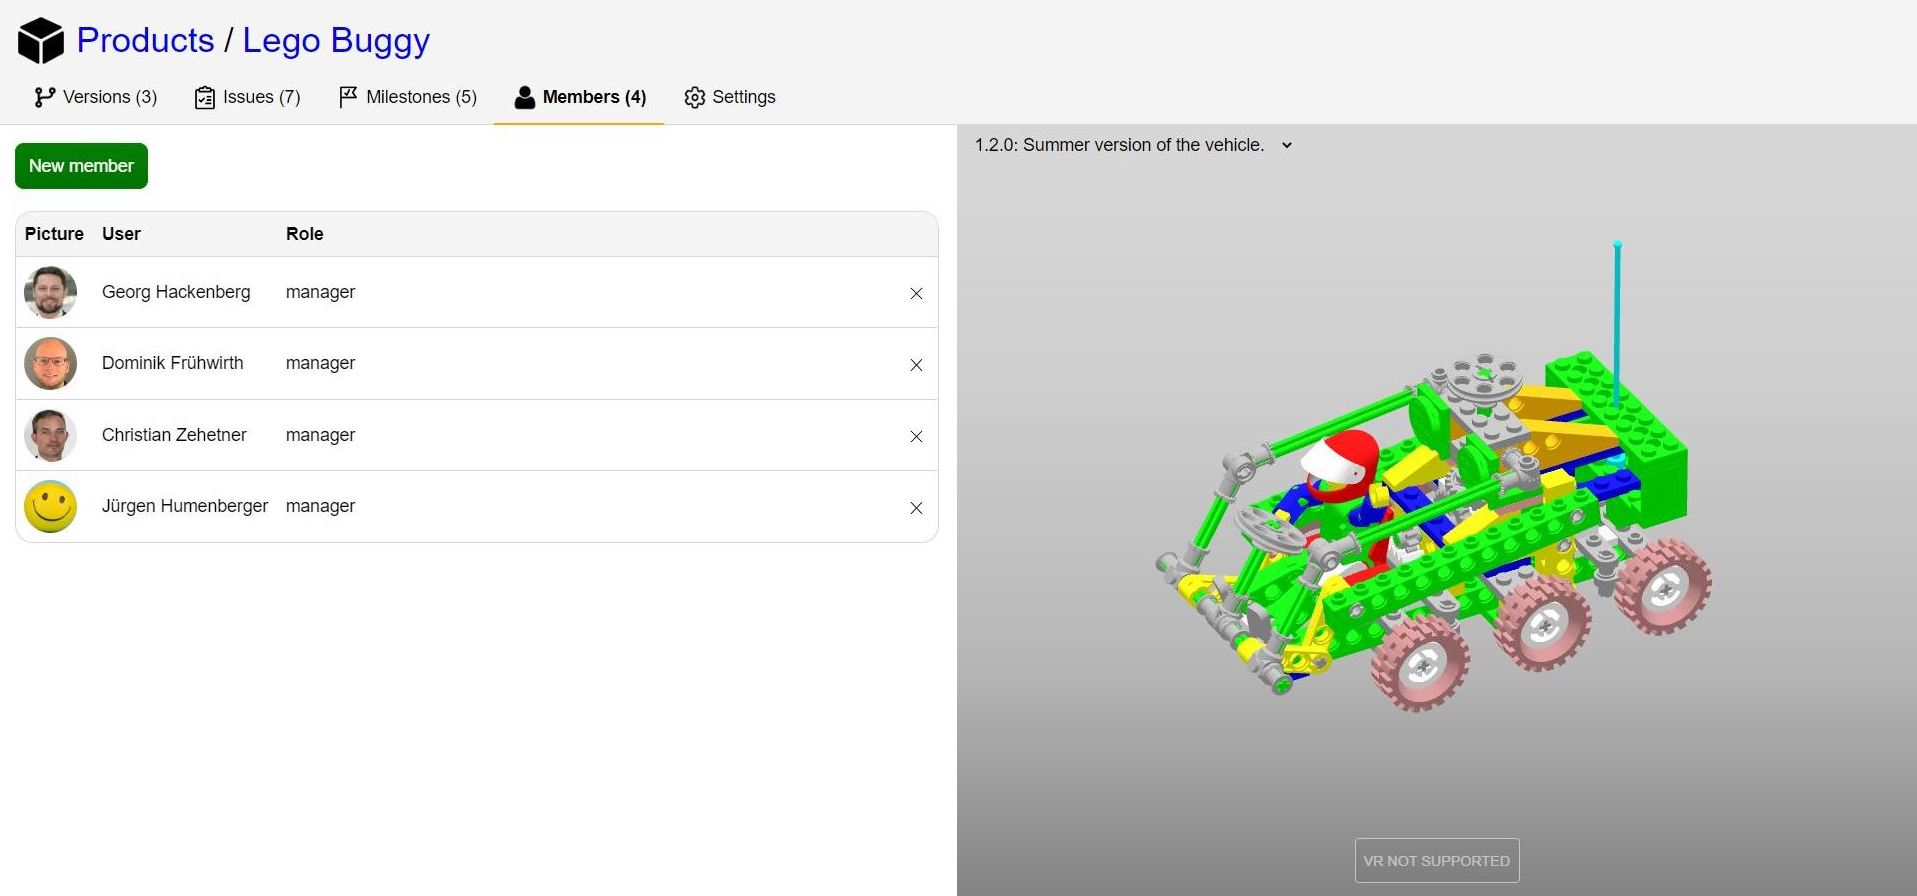
\includegraphics[width=\columnwidth]{memberview.JPG}
        \caption{Member view}
        \label{fig: memberview}
    \end{figure}

    \begin{figure}[h]
        \centering
        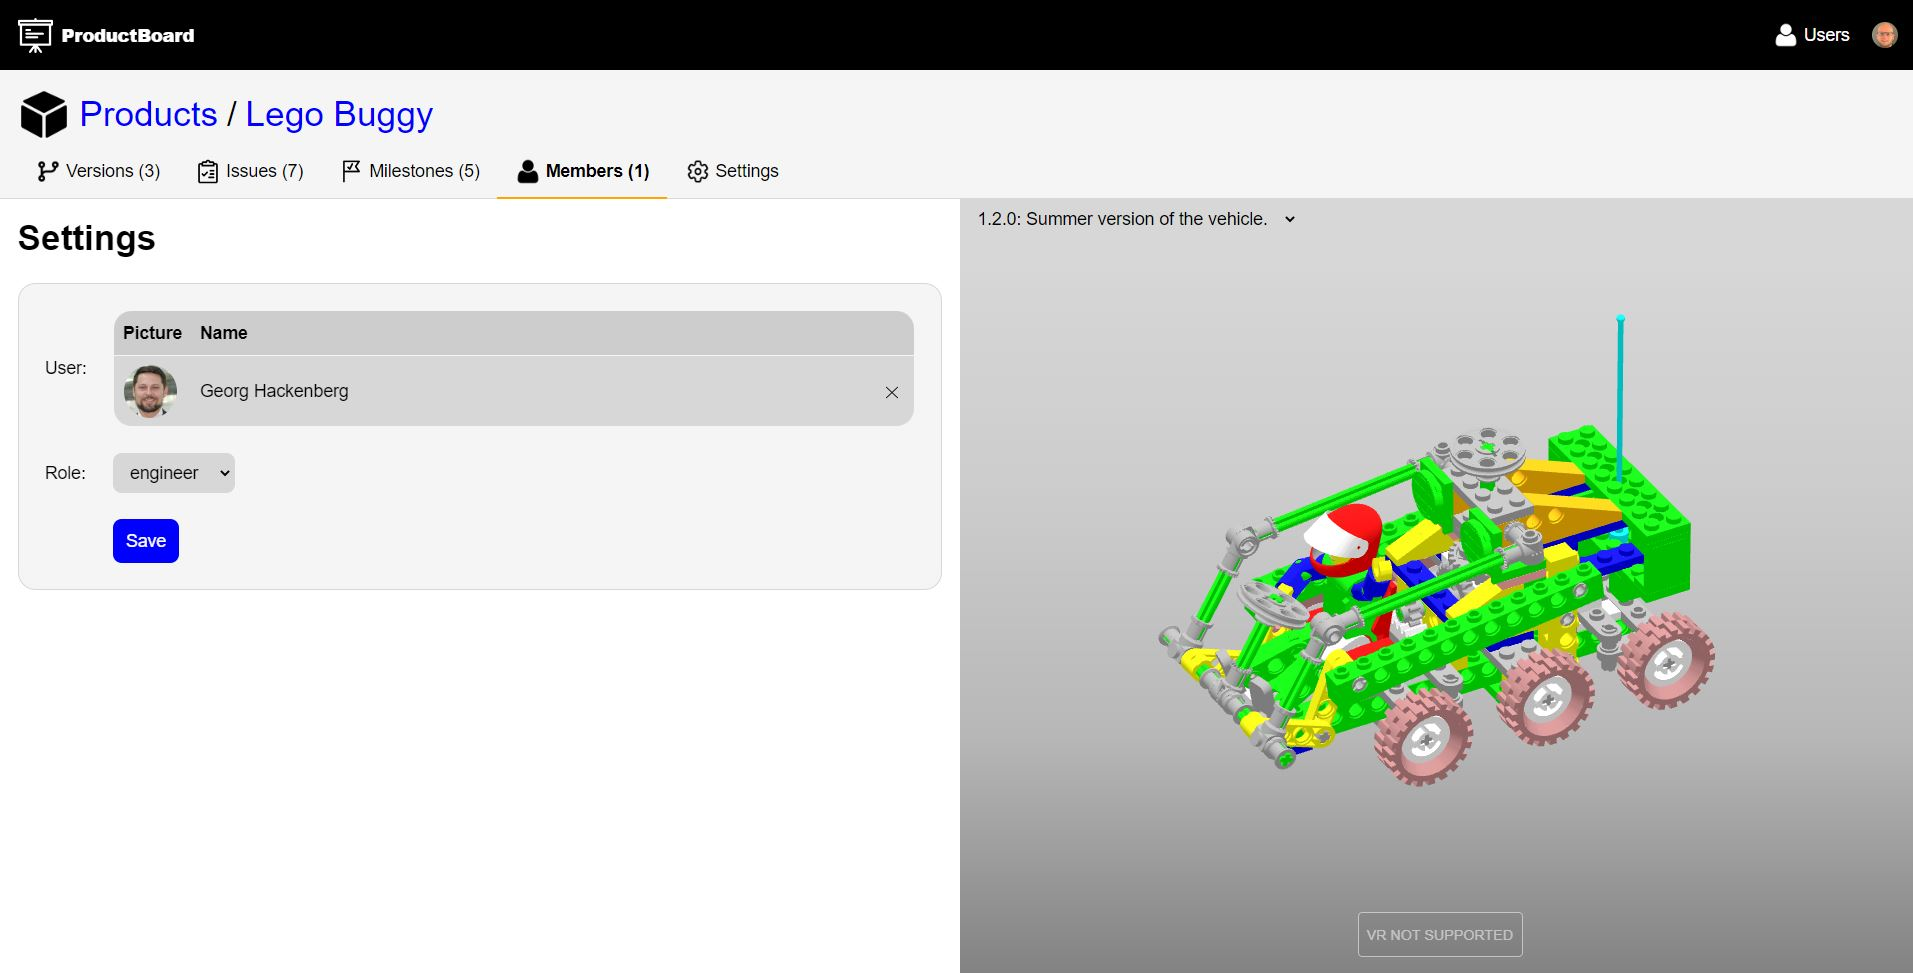
\includegraphics[width=\columnwidth]{membersettingsview.JPG}
        \caption{Membersettings view}
        \label{fig: membersettingsview}
    \end{figure}

    \subsubsection*{Productsettings view}
    In this view the attributes Name and Description of the selected product can be changed [see Fig. \ref{fig: productsettingsview} on page~\pageref{fig: productsettingsview}]. After clicking the Save button the changes are visible in the product overview
    \begin{figure}[h]
        \centering
        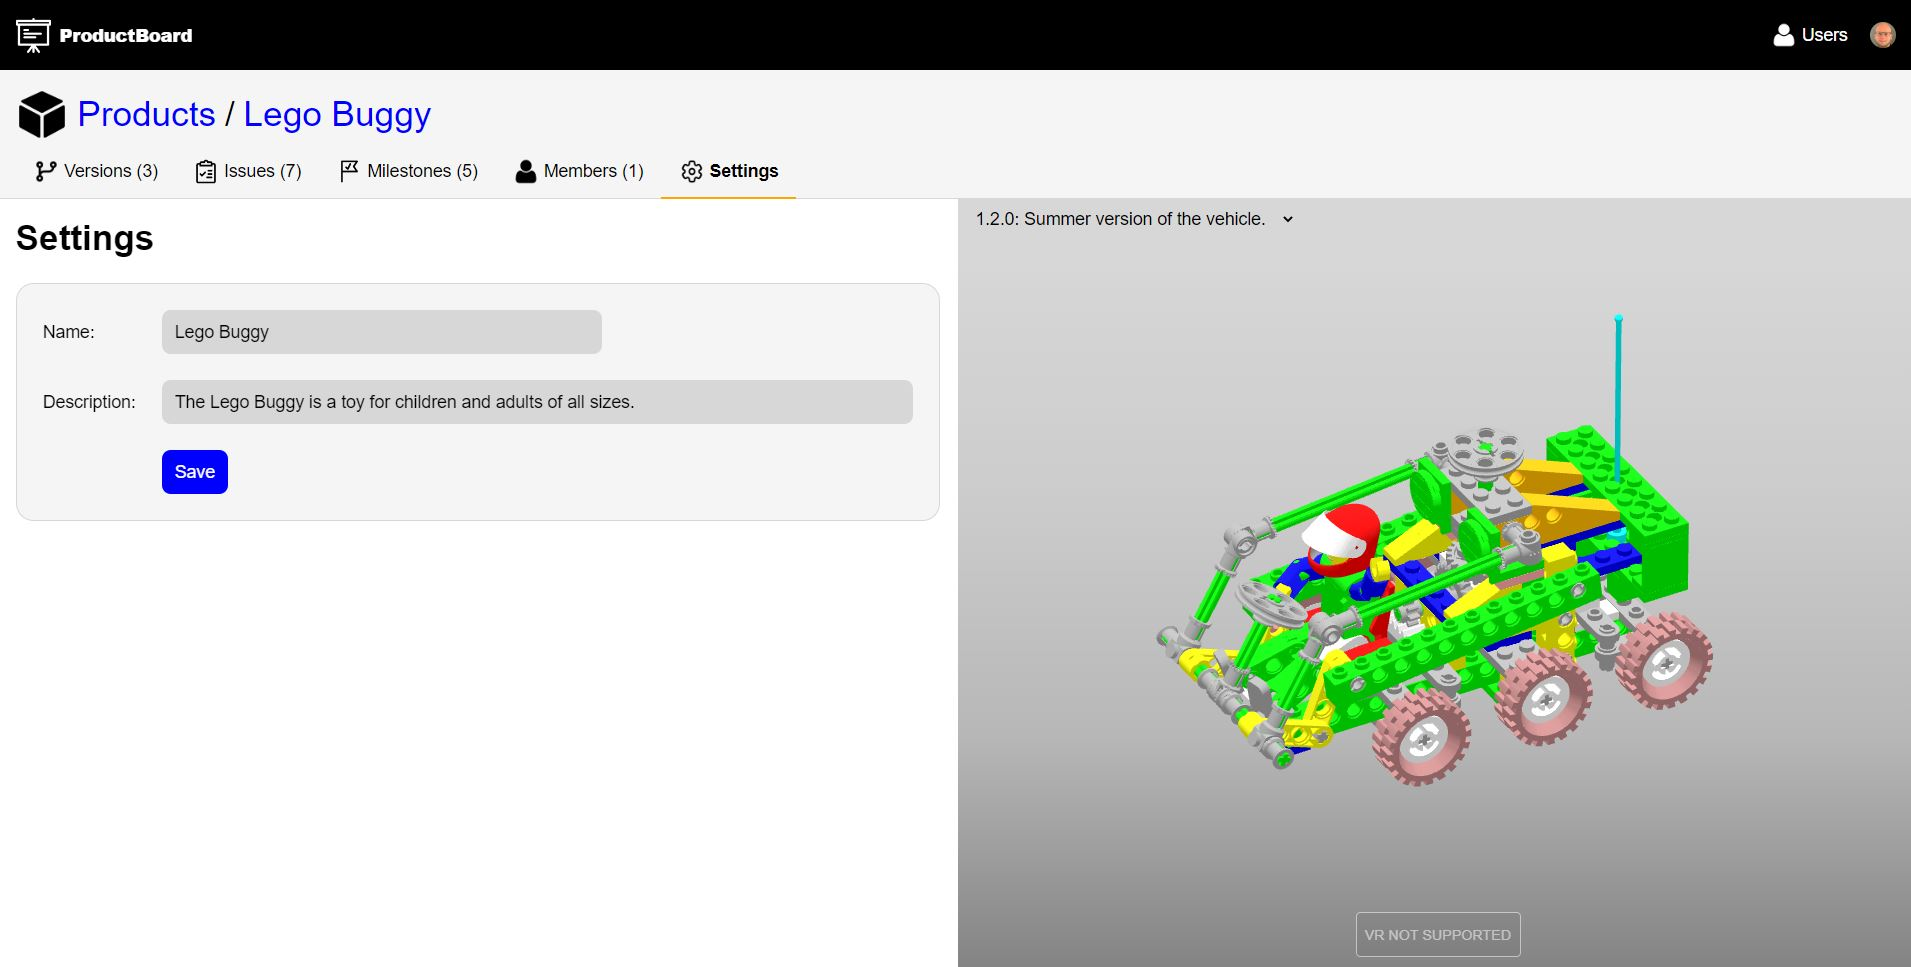
\includegraphics[width=\columnwidth]{productsettingsview.JPG}
        \caption{Productsettings view}
        \label{fig: productsettingsview}
    \end{figure}
    \section{Critical evaluation}
\label{sec:evaluation}
To solve the issues defined at the beginning of the article, we have developed the software ProductBoard. This software combines agile project management with product development. It was developed as a team of two people and the development time is currently one year. Due to the short development time, the software has of course not yet reached its final state. Nevertheless, it already covers a wide range of required issues. The development was done with state-of-the-art technology. The clean software architecture makes it easy to extend and maintain the software. As a single user, the software could already be tested at this stage. The user interface is responsive, and the software is intuitive to use. At this point, the app is still designed for a single user. There are still no functionalities built in that several PCs can access the data system simultaneously. This requires a revision in the backend to be able to react live to changes and display them again in the frontend. Another issue is that the data is consistent across all clients. One solution is a server client architecture with a web socket. For an adaptation to the customer, the permission system must also be adapted individually. Furthermore, the software has to be tested for stability. The current state of the project shows that it is possible and realistic to generate a benefit for agile product management and product development. In the next steps, the app can be made ready to enable communication between multiple clients. For this purpose, the current state can be continued and further developed without a complete revision. 

\section{Conclusion}
\label{sec:conclusion}

\subsection*{Summary}
To create a common basis for product development and product management, the software ProductBoard was developed. The advantage of this combination is that no engineering artifacts are lost. By bundling on a single app, a better overview of the process and more transparency is created. The customer can participate in agile product management and at the same time has the current status of all versions of the products. For this purpose, users can create and manage products on the platform. These products have versions, issues, comments and milestones. Members can also be added to the products, which have different permissions. There are three roles: manger, engineer and customer. The software offers versioning similar to GitHub. Based on the previous version and the current version, the history can be displayed graphically. Via issues, it is possible to assign tasks to one or more assignees. These tasks can be discussed in the associated conversation channel. After completion of a task, it can be marked as closed. Milestones are used to create an overview of the issues. Through the milestones the progress of the project can be tracked well. For the development of the software we decided to use tools from web development. This enables a cross-operating system user experience and can be well-built on a client server architecture. The three main components are the backend, the frontend and the database. In the center is the data model and the API for read and write operations to the data model. The frontend serves as a generic layer for triggering  operations and as a graphical representation of data. To enable operation on company and customer level a permission model was implemented. This can be customized according to the customer's needs by adjusting the customer's permissions individually. The functionality from the user's point of view was tested each time a new functionality was added. The tests have shown us that it is already possible to manage products on a PC using the software. In order to be ready for a wider range of users, the app still needs to be adapted. Due to the clear separation of frontend and backend, it is possible to extend the app in this direction without major reconstruction measures. 

\subsection*{Outlook}
According to our tests, the app has the potential to generate real added value for customers and companies. In order for the app to run on multiple devices at the same time and access a central backend, adjustments still need to be made. Furthermore, it has to be ensured that the software runs stable independent of all user inputs. This will be checked in a test phase. The architecture of the software was designed in such a way that other files can be uploaded in the future instead of CAD data. We plan to expand the scope of the app in the future. One idea is for example the management of electrical schematics. Like 3D CAD files, these can be designed and evaluated according to customer requirements. The software can also evolve in the direction of a simulation platform. It would be possible to upload entire simulated processes and support them with project management tools. For example, mechanical or electrical systems could be simulated directly in the View. For this, only the 3D view would have to be replaced by the corresponding functionality. Furthermore, we see potential in VR applications. With the help of VR, communication between companies and customers could be greatly improved during the project phase. The customer would have the possibility to view the 3D CAD model with all its versions in virtual space. This would allow the customer to move the model freely in space and thus capture even more engineering artifacts. These functions are already partially implemented in the software and will be extended in the future. A follow-up project is already in the planning phase and will be launched in the next few months. The follow-up project will complement this software with VR functions to enable an evaluation of the product development process in virtual space. 

    \bibliographystyle{plain}
    \bibliography{main}

 
\end{document}